%% ----------------------------------------------------------------
%% Thesis.tex -- MAIN FILE (the one that you compile with LaTeX)
%% ----------------------------------------------------------------
% Set up the document
\documentclass[a4paper, 11pt, oneside]{Thesis}  % Use the "Thesis" style, based on the ECS Thesis style by Steve Gunn
\graphicspath{Figures/}  % Location of the graphics files (set up for graphics to be in PDF format)
% Include any extra LaTeX packages required
\usepackage{changepage}
\usepackage{fancyhdr}
\usepackage{float}
\usepackage{import}
\usepackage{lipsum}
\usepackage[square, numbers, comma, sort&compress]{natbib}  % Use the "Natbib" style for the references in the Bibliography
\usepackage{setspace}
\hypersetup{urlcolor=blue, colorlinks=true}  % Colours hyperlinks in blue, but this can be distracting if there are many links.
\usepackage{vector}  % Allows "\bvec{}" and "\buvec{}" for "blackboard" style bold vectors in maths
\usepackage{verbatim}  % Needed for the "comment" environment to make LaTeX comments
\usepackage{subfig}
\usepackage{graphicx}
\usepackage{gensymb}
\usepackage{afterpage, geometry, pdflscape, tabularx, ulem} % for landscape tables
\usepackage{multirow}
\usepackage{pdfpages}
\usepackage[usenames,dvipsnames]{xcolor}
\usepackage{afterpage}

\definecolor{ForestGreen}{RGB}{34, 139, 34}
\definecolor{Rhodamine}{RGB}{188, 82, 134}

\newgeometry{left=2in,right=0in,bottom=0in,top=2in}

% Use this to change the margin width for a snippet of text/table/figure etc.
\def\changemargin#1#2{\list{}{\rightmargin#2\leftmargin#1}\item[]}
\let\endchangemargin=\endlist

%\def \thesistitle{Sensing and Actuation in Conductive Particle Electroactive Elastomeric Bodies}
\def \thesistitle{Integration of Biomimetic Pressure Mapping and Actuation in Soft Electroactive Elastomer Composites}
%\def \thesistitle{Integrated sensing and actuation in stretchable devices - EIT and EAP integration}
%\def \thesistitle{Electrical impedance tomography based pressure mapping integration with dielectric elastomer actuators using conductive particle elastomer composites.}
%\def \thesistitle{Synergy Between Sensing and Actuation: Electroactive Elastomeric Composite Bodies for Soft Robotics.}
%\def \thesistitle{The Interplay of Two Soft Robotics Sensor and Actuator Technologies using Carbon Based Elastomer Composites.}
%\def \thesistitle{Beyond Rigid: Forming and Characterising Novel Soft Sensor-Actuator Technologies.}
%\def \thesistitle{Towards Artificial Skin and Muscle: Soft Electroactive Elastomeric Bodies that Can Sense and Contract}

%% ----------------------------------------------------------------
\begin{document}
	\frontmatter      % Begin Roman style (i, ii, iii, iv...) page numbering
	% Set up the Title Page
	\title  {\thesistitle}
	\authors  {\texorpdfstring
		{\href{ellingham.richie@gmail.com}{Richard James Morrin Ellingham}}
		{Richard James Morrin Ellingham}
	}
	\addresses  {\groupname\\\deptname\\\univname}  % Do not change this here, instead these must be set in the "Thesis.cls" file, please look through it instead
	\date       {\today}
	\subject    {}
	\keywords   {}
	\maketitle
	%% ----------------------------------------------------------------
	\setstretch{1.5}  % It is better to have smaller font and larger line spacing than the other way round
	% Define the page headers using the FancyHdr package and set up for one-sided printing
	\fancyhead{}  % Clears all page headers and footers
	\rhead{\thepage}  % Sets the right side header to show the page number
	\lhead{}  % Clears the left side page header
	\pagestyle{fancy}  % Finally, use the "fancy" page style to implement the FancyHdr headers
	%% ----------------------------------------------------------------
	% Declaration Page required for the Thesis, your institution may give you a different text to place here
	\Declaration{
		\addtocontents{toc}{\vspace{1em}}  % Add a gap in the Contents, for aesthetics
		I, AUTHOR NAME, declare that this thesis titled, `\thesistitle' and the work presented in it are my own. I confirm that:
		\begin{itemize}
			\item[\tiny{$\blacksquare$}] This work was done wholly or mainly while in candidature for a research degree at this University.
			\item[\tiny{$\blacksquare$}] Where any part of this thesis has previously been submitted for a degree or any other qualification at this University or any other institution, this has been clearly stated.
			\item[\tiny{$\blacksquare$}] Where I have consulted the published work of others, this is always clearly attributed.
			\item[\tiny{$\blacksquare$}] Where I have quoted from the work of others, the source is always given. With the exception of such quotations, this thesis is entirely my own work.
			\item[\tiny{$\blacksquare$}] I have acknowledged all main sources of help.
			\item[\tiny{$\blacksquare$}] Where the thesis is based on work done by myself jointly with others, I have made clear exactly what was done by others and what I have contributed myself.
			\\
		\end{itemize}
		Signed: \\
		\rule[1em]{25em}{0.5pt}  % This prints a line for the signature
		Date: \\
		\rule[1em]{25em}{0.5pt}  % This prints a line to write the date
	}
	\clearpage  % Declaration ended, now start a new page
	%% ----------------------------------------------------------------
	% The "Funny Quote Page"
	\pagestyle{empty}  % No headers or footers for the following pages
	\null\vfill
	% Now comes the "Funny Quote", written in italics
%	\textit{``PHD stands for Permanent Head Damage''}
	\textit{``We've made good progress with the brains of robots but their bodies are still primitive. We need a new kind of robot body that is inspired by elegance, efficiency, and by the soft materials found in nature. Indeed, this has become the key idea of a new field of research called soft robotics.''}
	\begin{flushright}
		C. Keplinger, 2019
	\end{flushright}
	\vfill\vfill\vfill\vfill\vfill\vfill\null
	\clearpage  % Funny Quote page ended, start a new page
	\setstretch{1.0}
	%% ----------------------------------------------------------------
	% The Abstract Page
	\addtotoc{Abstract}  % Add the "Abstract" page entry to the Contents
	\abstract{\addtocontents{toc}{\vspace{1em}}  % Add a gap in the Contents, for aesthetics
		% 
	Some of the world's most advanced technology is rigid due to various factors such as; manufacturability, miniaturisability, physical linearity, and more ideal linear physical mechanics. Rigid mechanisms were engineered first and have been refined to a high level, but now are encountering limitations leading to demand for soft robotic solutions that mimic biological evolution. This thesis develops and integrates an artificial skin and artificial muscle technology by combining of Electrical Impedance Tomography (EIT), carbon black silicone rubber (CBSR) elastomer composites, and Dielectric Elastomer Actuators (DEAs) to enhance pressure mapping, strain sensing, and actuation capabilities. 
	CBSR elastomer composites, noted for their high stretchability, piezoresistivity, and biocompatibility, were investigated to understand their non-linear time dependent phenomena in particular, resistance relaxation behavior. This research contributes to optimising the design of flexible dynamic strain sensors by modelling the response of resistance to transient strain inputs. The next part of the thesis describes development of an EIT-based pressure mapping system using a CBSR sensing domain that mimics pressure mapping qualities of human skin. This system was evaluated for its spatial and temporal resolution, showing potential for creating artificial pressure-sensitive skin with practical applications. At the core of this thesis the integration of EIT-based sensing with DEAs was tested and analysed to improve the mapping of compressive forces across the actuator electrode surfaces. Despite some trade-offs in accuracy due to electrode compliance, this approach offers promising advancements for applications requiring precise actuation and pressure mapping. This work has contributed towards filing a patent for an DEA-EIT actuator-sensor device. Additionally, the research has uncovered unintentional power generation in DEA-EIT systems through FEA studies and analytical validation, which could function as Dielectric Elastomer Generators (DEGs) with mapped compressive load inputs. This finding highlights the multi-functionality of DEAs and suggests opportunities for energy harvesting applications. To aid the portability of EIT-based pressure mapping sensor developed, a low-cost circuit and evaluation tools were developed. This system enables comprehensive characterisation of various sensing domains and supports advancements in EIT-based soft sensor technology, with implications for biomedical devices, robotics, and energy harvesting. 
	Overall, this thesis advances the field of soft sensors by investigating an electroactive material and using the material to integrate EIT-based pressure mapping with dielectric elastomer actuator technologies, providing new insights and applications in dynamic sensing and actuation.
	}
	\clearpage  % Abstract ended, start a new page
	%% ----------------------------------------------------------------
	\setstretch{1.3}  % Reset the line-spacing to 1.3 for body text (if it has changed)
	% The Acknowledgements page, for thanking everyone
	\acknowledgements{
		\addtocontents{toc}{\vspace{1em}}  % Add a gap in the Contents, for aesthetics
	I would like to thank many people who have implicitly and explicitly helped me get through my doctorate. First, the UC Bioengineering office including the Lung Ladies, Lung lads, IPC, Hamish for infinite Friday beers, and Nic's abstract art. Also included in the office, Geoff Chase, for a constant stream of stories and advice always within earshot. The Mechanical Engineering post-grad office for baking, fruit, and comic relief. The UC Mechanical and Electrical department technicians for yarns and practical advice. All of the students and project groups I tutored and mentored, keeping me on my toes throughout the doctorate. Thanks for the motivation from all of my friends with the never-ending question `so... when do you finish', a very motivating and difficult question answer. Something that prolonged the journey but kept me sane, were the technical the side jobs and fun adventures with colleagues and friends maintaining my sanity. A special thanks to my supervision and collaborations abroad, including my materials science work in IMDEA with Juan Jose and Anastasia and my time with with the MEiTNER soft robotics research group led by Markus Vorrath. Thanks to my internal supervision from Tim teaching me what PHD stands for and my co-supervisors Chris and Lui who have been a good source of advice, yarns, and general guidance. A thank you to my family for being supportive in times of strife. Finally, I would like to thank my partner Tess for her ongoing support and distractions from my PhD work.
	}
	\clearpage  % End of the Acknowledgements
	%% ----------------------------------------------------------------
	\pagestyle{fancy}  %The page style headers have been "empty" all this time, now use the "fancy" headers as defined before to bring them back
	%% ----------------------------------------------------------------
	\lhead{\emph{Contents}}  % Set the left side page header to "Contents"
	\tableofcontents  % Write out the Table of Contents
	%% ----------------------------------------------------------------
	\lhead{\emph{List of Figures}}  % Set the left side page header to "List if Figures"
	\listoffigures  % Write out the List of Figures
	%% ----------------------------------------------------------------
	\lhead{\emph{List of Tables}}  % Set the left side page header to "List of Tables"
	\listoftables  % Write out the List of Tables
	%% ----------------------------------------------------------------
	\setstretch{1.5}  % Set the line spacing to 1.5, this makes the following tables easier to read
	\clearpage  % Start a new page
	\vspace{-1cm}
	\lhead{\emph{Abbreviations}}  % Set the left side page header to "Abbreviations"
	\vspace{-0.5cm}
	\listofsymbols{ll}  % Include a list of Abbreviations (a table of two columns)
	{
		% \textbf{Acronym} & \textbf{W}hat (it) \textbf{S}tands \textbf{F}or \\
		\textbf{ADC} & \textbf{A}nalog-\textbf{t}o-\textbf{D}igital \textbf{C}onverter \\
		\textbf{CAD} & \textbf{C}omputer \textbf{A}ided \textbf{D}esign \\
		\textbf{CB} & \textbf{C}arbon \textbf{B}lack \\
		\textbf{CE} & \textbf{C}ompliant \textbf{E}electrode \\
		\textbf{CFA} & \textbf{C}artesian \textbf{F}orce \textbf{A}pplicator \\
		\textbf{CoM} & \textbf{C}enter of \textbf{M}ass \\
		\textbf{CPEC} & \textbf{C}onductive \textbf{P}article \textbf{E}lastomer \textbf{C}omposite\\
		\textbf{DE} & \textbf{D}ielectric \textbf{E}lastomer \\
		\textbf{DEA} & \textbf{D}ielectric \textbf{E}lastomer \textbf{A}ctuator \\
		\textbf{DEG} & \textbf{D}ielectric \textbf{E}lastomer \textbf{G}enerator \\
		\textbf{DUT} & \textbf{D}omain \textbf{U}nder \textbf{T}est \\
		\textbf{EIT} & \textbf{E}lectrical \textbf{I}mpedance \textbf{T}omography \\
		\textbf{ERT} & \textbf{E}lectrical \textbf{R}esistance \textbf{T}omography \\
		\textbf{FEA} & \textbf{F}inite \textbf{E}lement \textbf{A}nalysis \\
		\textbf{FEM} & \textbf{F}inite \textbf{E}lement \textbf{M}odelling \\
		\textbf{FPC} & \textbf{F}lexible \textbf{P}rinted \textbf{C}ircuit \\
		\textbf{MUX} & \textbf{M}ultiplexer \\
		\textbf{PCB} & \textbf{P}rinted \textbf{C}ircuit \textbf{B}oard \\
		\textbf{PCBA} & \textbf{P}rinted \textbf{C}ircuit \textbf{B}oard \textbf{A}ssembly\\
		\textbf{PDMS} & \textbf{P}oly\textbf{d}i\textbf{m}ethyl\textbf{s}iloxane (AKA silicone)\\
		\textbf{PNEC} & \textbf{P}iezoresistive \textbf{N}anoparticle \textbf{E}lastomer \textbf{C}omposite\\
		\textbf{SMU} & \textbf{S}ource \textbf{M}easure \textbf{U}nit \\
		\textbf{SMD} & \textbf{S}urface-\textbf{M}ount \textbf{D}evice \\
		\textbf{SR} & \textbf{S}ilicone \textbf{R}ubber \\
		\textbf{EAP} & \textbf{E}lectro-\textbf{A}ctive \textbf{P}olymer\\

	}
	%% ----------------------------------------------------------------
	
	\clearpage  %Start a new page
	\lhead{\emph{Nomenclature}}  % Set the left side page header to "Symbols"
	\listofnomenclature{lll}  % Include a list of Symbols (a three column table)
	{
		% symbol & name & unit \\
		$A$ & Area & [m$^2$] \\
		$C$ & Capacitance & [F] \\
		$\epsilon_0$ & Vacuum Permittivity & [Fm$^{-1}$] \\
		$\epsilon_r$ & Relative Permittivity & [a.u.] \\
		$K$ & Bulk Modulus & [Pa] \\
		$\nu$ & Poisson’s Ratio & [a.u.] \\
		$Q$ & Electrical Charge & [C] \\
		$U_E$ & Electrical Potential Energy & [J] \\
		$U_{\epsilon}$ & Elastic Potential Energy & [J] \\
		$R$ & Resistance & [$\Omega$] \\
		$\sigma$ & Stress & [Pa] \\
		$S$ or $\varepsilon$ & Strain & [a.u. or \%] \\ % change this to S or \varepsilon?
		$\dot\varepsilon$ & Strain Rate & [\%s$^{-1}$] \\
		$V$ & Voltage & [V] \\
		$Y$ or $E$ & Young's Modulus & [Pa] \\
		$z$ or $d$ & Thickness & [m] \\

		
	}
	%% ----------------------------------------------------------------
	% End of the pre-able, contents and lists of things
	% Begin the Dedication page
	\setstretch{1.5}  % Return the line spacing back
	\pagestyle{empty}  % Page style needs to be empty for this page
	\dedicatory{Dedicated to tinned baked beans in all their glory\ldots}
	\addtocontents{toc}{\vspace{2em}}  % Add a gap in the Contents, for aesthetics
	%% ----------------------------------------------------------------
	\mainmatter	  % Begin normal, numeric (1,2,3...) page numbering
	\pagestyle{fancy}  % Return the page headers back to the "fancy" style
	% Include the chapters of the thesis, as separate files
	% Just uncomment the lines as you write the chapters
	\lhead{\emph{\chapiname}}
	\import{Chapters/}{Chapter1.tex} % Introduction
	\lhead{\emph{\chapiiname}}
	\import{Chapters/}{Chapter2.tex} % Literature Review
	\lhead{\emph{\chapiiiname}}
	\import{Chapters/}{Chapter3.tex} % CBSR behaviour
	\lhead{\emph{\chapivname}}
	\import{Chapters/}{Chapter4.tex} % Improved EIT-based sensor
	\lhead{\emph{\chapvname}}
	\import{Chapters/}{Chapter5.tex} % Portable EIT hardware 
	\lhead{\emph{\chapviname}}
	\import{Chapters/}{Chapter6.tex} % DEA-EIT
	\lhead{\emph{\chapviiname}}
	\import{Chapters/}{Chapter7.tex} % DEA-EIT an unintended DEG
	\lhead{\emph{\chapviiiname}}
	\import{Chapters/}{Chapter8.tex} % Discussion and Conclusion

	%% ----------------------------------------------------------------
	% Now begin the Appendices, including them as separate files
	\addtocontents{toc}{\vspace{2em}} % Add a gap in the Contents, for aesthetics
	\appendix % Cue to tell LaTeX that the following 'chapters' are Appendices
	\chapter{Thesis Crossword}
\label{appendix-A}
\vspace{-2cm}
\begin{table}[H]
	\centering
	\begin{tabular}{p{\linewidth}}
		\hspace{1cm}
		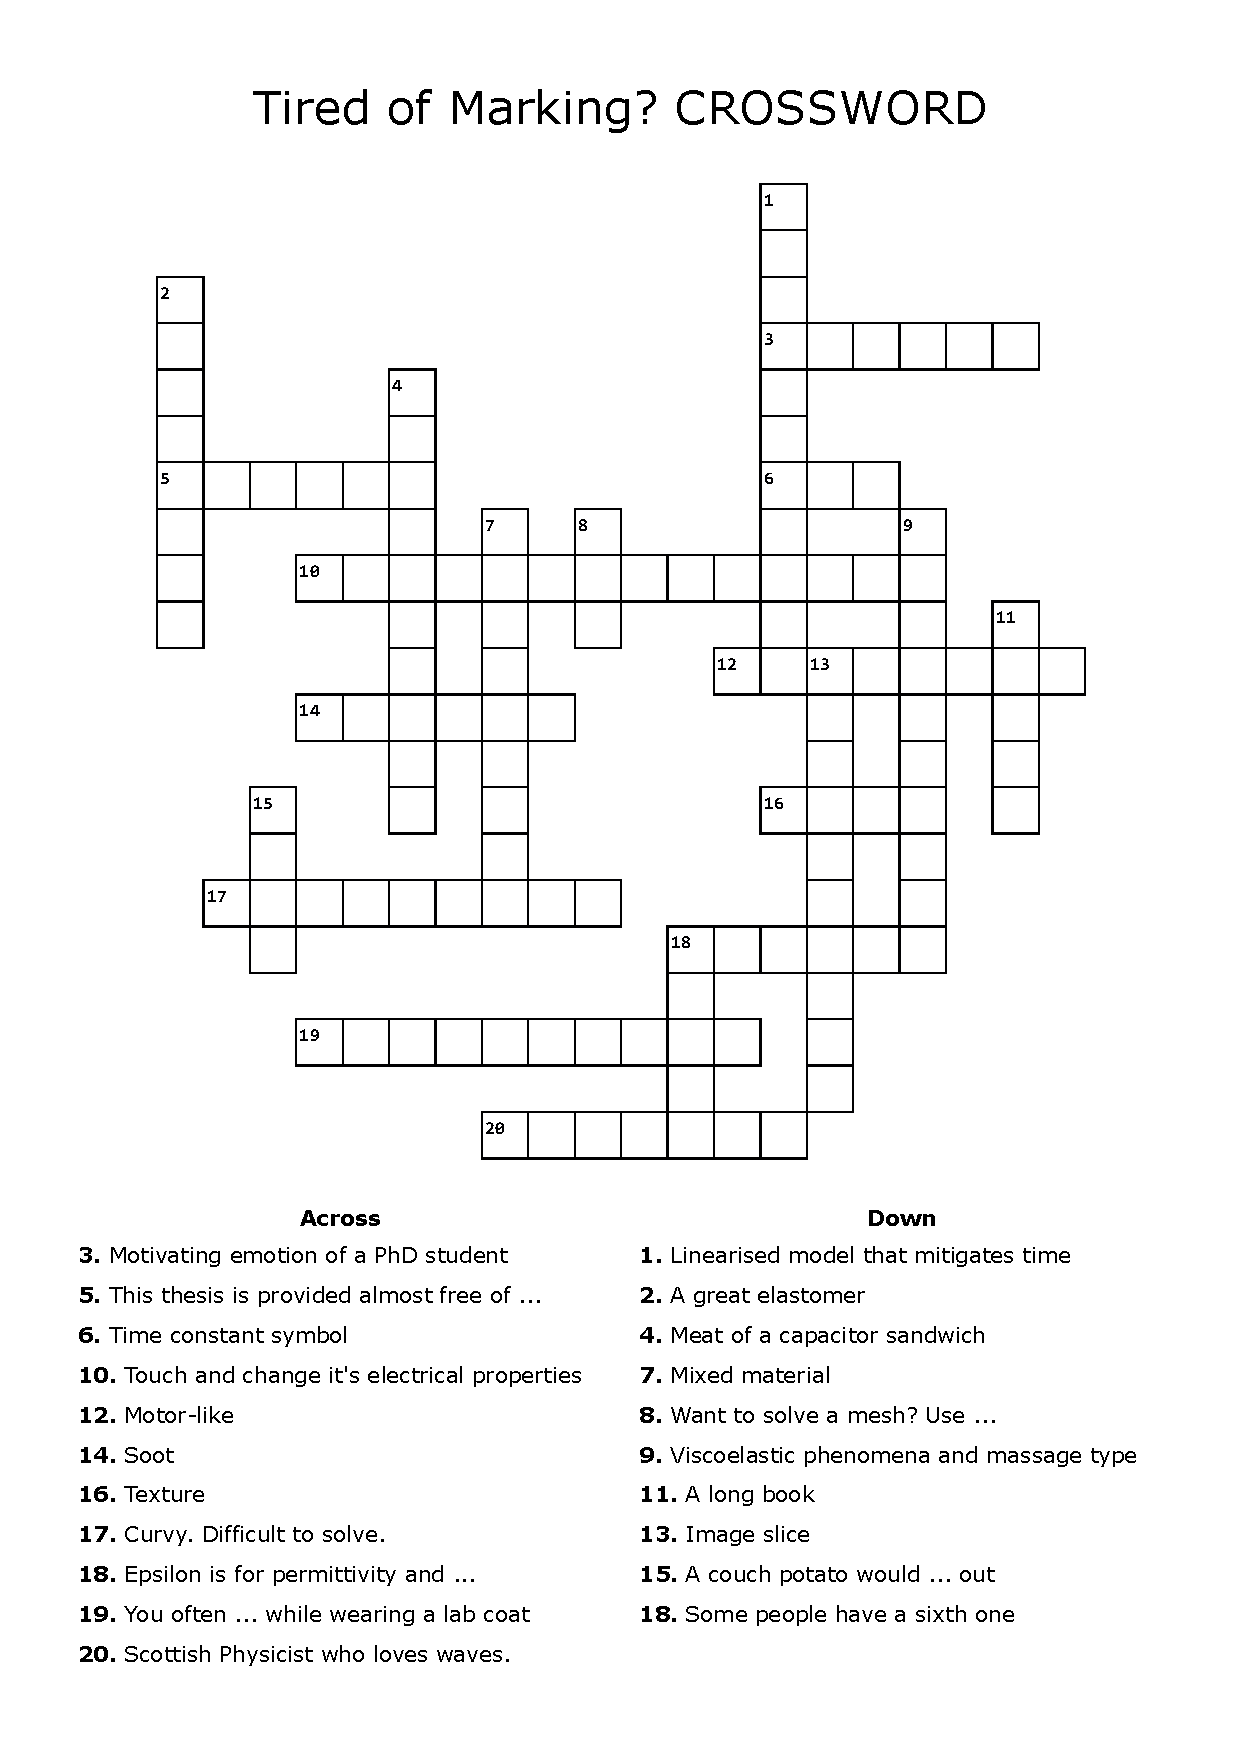
\includegraphics[width=0.85\linewidth]{fun-thesis-crossword.pdf}
	\end{tabular}
\end{table}
%\includepdf[pages=-,scale=0.2,offset=70 0]{}

	\chapter{Strain-Stress-Resistance Experiments}
\label{appendix-B}
%\section{title}
\begin{figure}[H]
	\centering
	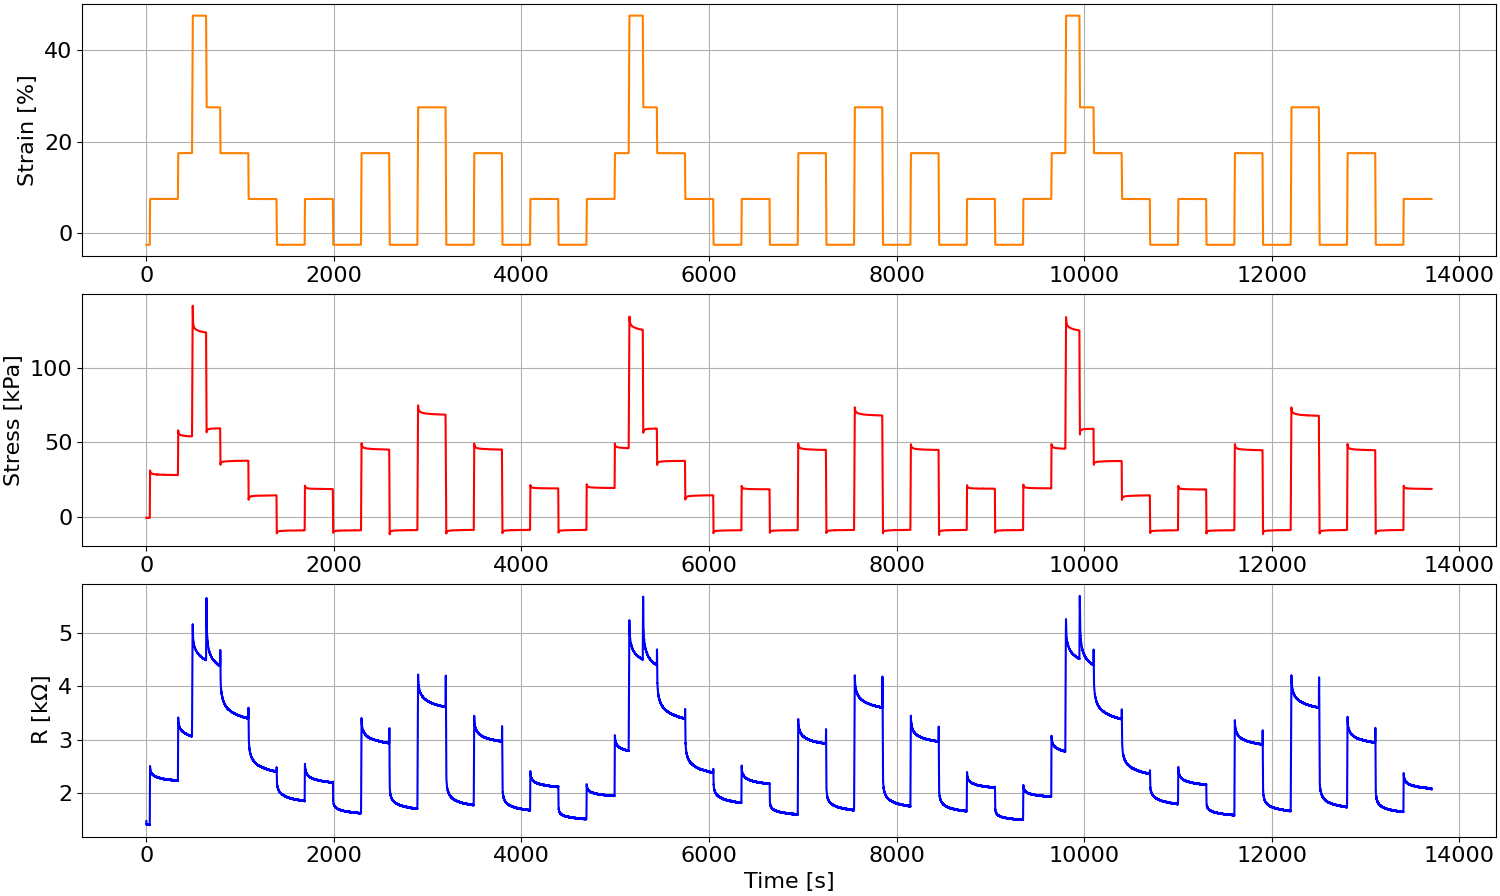
\includegraphics[width=\linewidth]{Figures/2_7-5_E4pin_20mm_v12_0.1_0.2_0.3_strain_1mm_offset_erroneous.png}
	\caption{Strain test sequence showing the shoulder phenomena correlation for varying magnitudes of strain for a 7.5 wt\% CBSR specimen dogbone sample. This experiment had an unintentional offset of 1 mm, however this showed a drastic decrease shoulder phenomena when the falling edge is crossing the x-axis.}
	\label{fig:strain-hill}
\end{figure}
\begin{figure}[H]
	\centering
	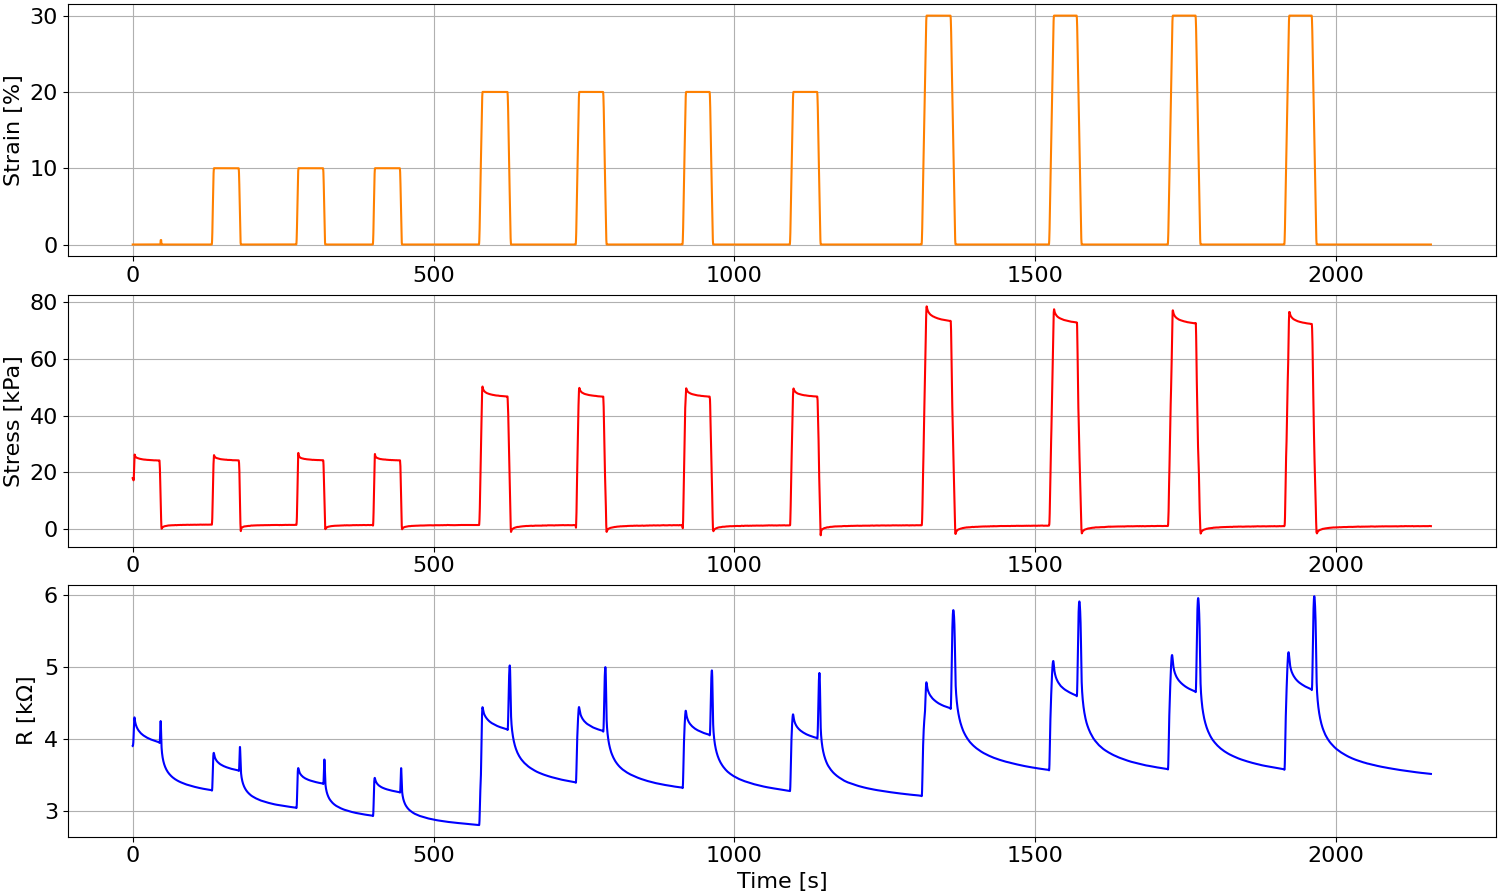
\includegraphics[width=\linewidth]{Figures/1_7-5_Epin_20mm_v2_DC_meas_3_strains.png}
	\caption{Strain test sequence showing the shoulder phenomena correlation for varying magnitudes of strain for a 7.5 wt\% CBSR specimen dogbone sample. This experiment used DC measurements, so the macro downward trend in resistance is more obvious than other experimental data given in this work with used a switched AC signal.}
	\label{fig:strain-train-DC-meas}
\end{figure}
\begin{figure}[H]
	\centering
	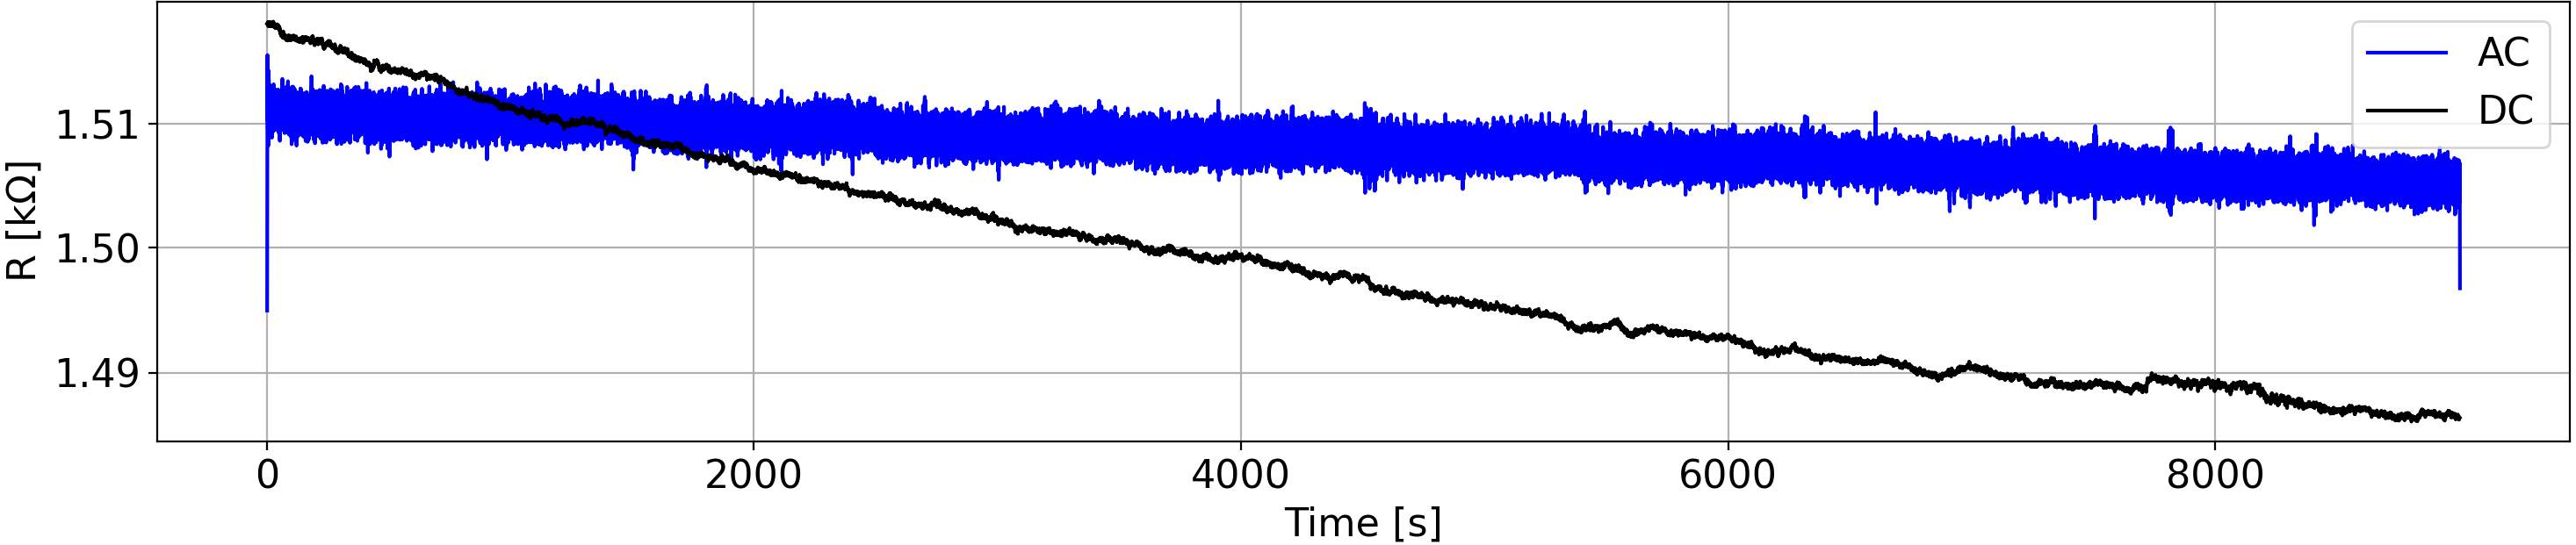
\includegraphics[width=\linewidth]{Figures/AC_vs_DC_long_decay_2_7-5_CBSR}
	\caption{AC vs DC downward trend in resistance for an unstrained 7.5 wt\% CBSR composite dogbone specimen.}
	\label{fig:res-AC-DC}
\end{figure}


	\chapter{Chapter Title}
\label{appendix-C}

	\chapter{EIT-based Pressure Sensor Performance Metrics}
\label{appendix-D}

\section{Noise Removal}
\begin{figure}[H]
	\centering
	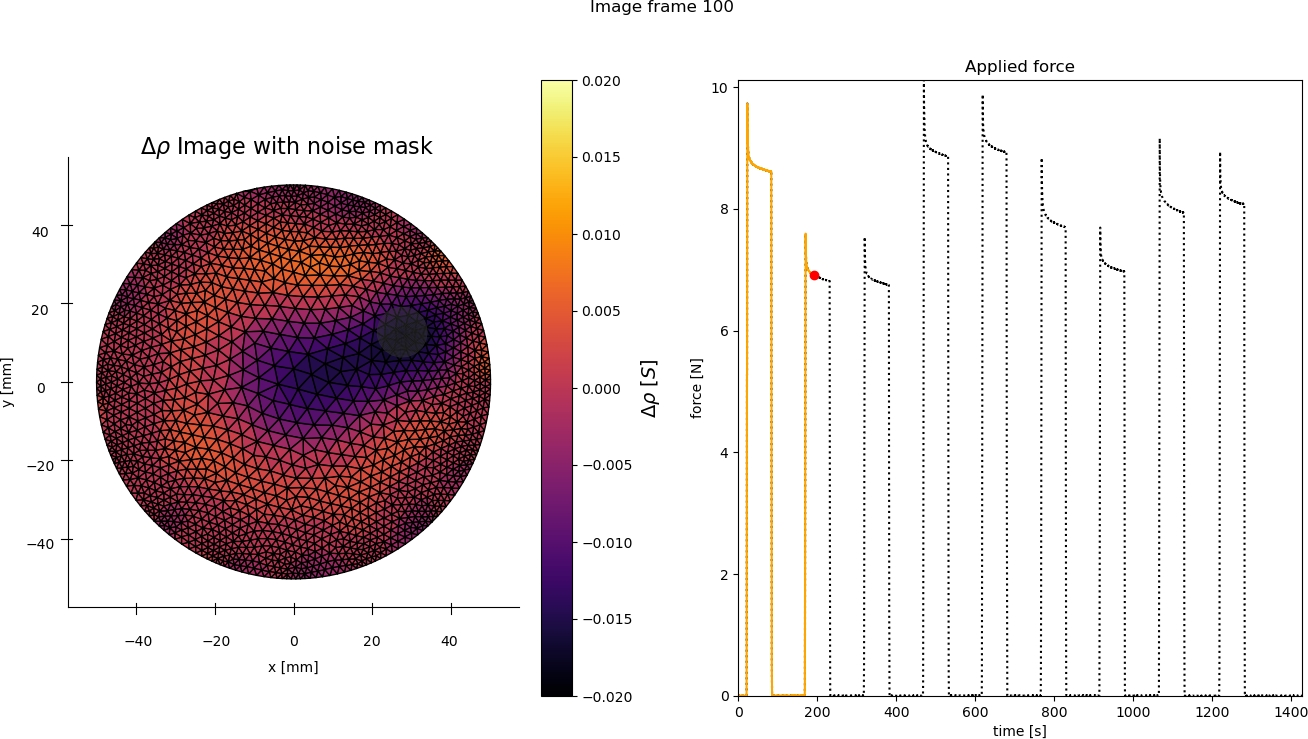
\includegraphics[width=\linewidth]{Figures/CBSR_9p_2_9push_25strain_60s_1mA_4_frame100_noise_mask.jpg}
	\caption{An experimental snapshot. Left: Before executing the performance metrics calculations, the noise floor mask was applied to the 9\% CBSR material. Right: Time series force data}
	\label{fig:noise_floor_mask_9p}
\end{figure}
\begin{figure}[H]
	\centering
	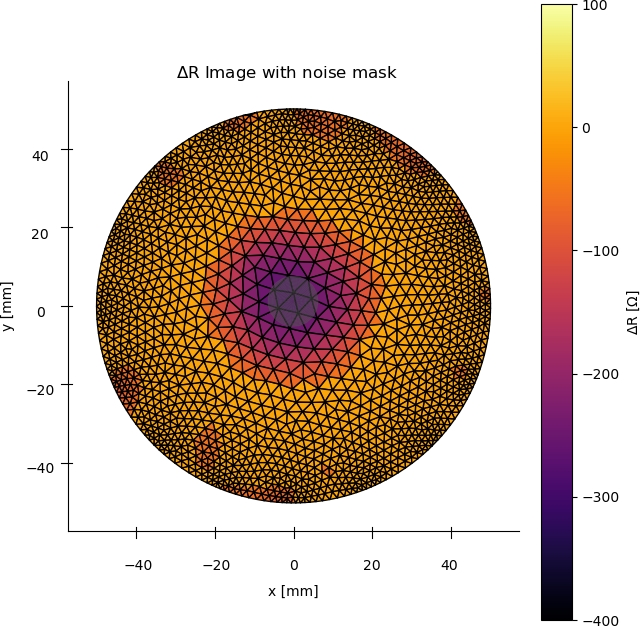
\includegraphics[width=0.6\linewidth]{Figures/CBSR_8p_9push_20strain_60s_4_frame20_noise_mask.jpg}
	\caption{Before executing the performance metrics calculations, the noise floor mask was applied to the 8\% CBSR material shown in Figure \ref{fig:CBSR sample and holder}}
	\label{fig:noise_floor_mask_8p}
\end{figure}


\section{More Threshold Percentage Masks}
\begin{figure}[H]
	\centering
	\begin{minipage}[t]{0.3\textwidth}
		\vspace{0pt}
		\subfloat[][]{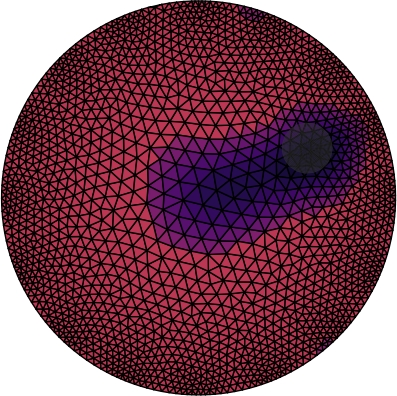
\includegraphics[width=\textwidth]{Figures/CBSR_9p_2_9push_25strain_60s_1mA_4_frame100_25p_mask_crop.jpg}\label{thresh25}}
		\vfill
		\subfloat[][]{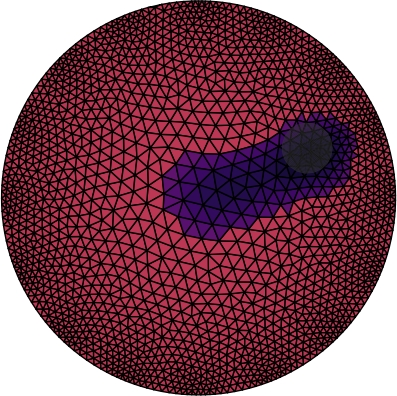
\includegraphics[width=\textwidth]{Figures/CBSR_9p_2_9push_25strain_60s_1mA_4_frame100_50p_mask_crop.jpg}\label{thresh50}}
		\vspace{0pt}
	\end{minipage}%
	\begin{minipage}[t]{0.3\textwidth}
		\vspace{0pt}
		\subfloat[][]{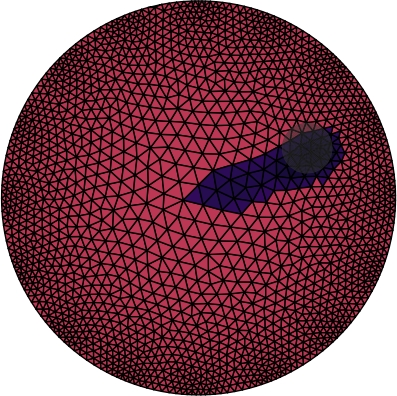
\includegraphics[width=\textwidth]{Figures/CBSR_9p_2_9push_25strain_60s_1mA_4_frame100_75p_mask_crop.jpg}\label{thresh75}}
		\vfill
		\subfloat[][]{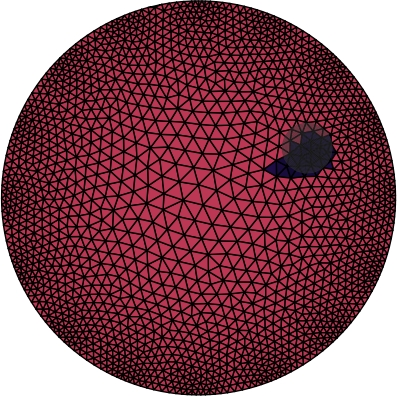
\includegraphics[width=\textwidth]{Figures/CBSR_9p_2_9push_25strain_60s_1mA_4_frame100_85p_mask_crop.jpg}\label{thresh85}}
		\hfill
	\end{minipage} 
	\begin{minipage}[t]{.1\textwidth}
		\vspace{0pt}
		\subfloat[][]{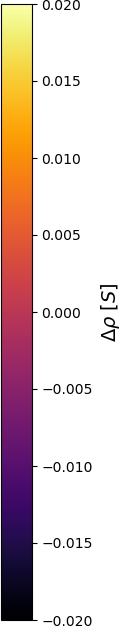
\includegraphics[width=\textwidth]{Figures/CBSR_9p_2_9push_25strain_60s_1mA_4_frame100_scale_bar.jpg}\label{colour_bar}}
		\hfill
	\end{minipage}  
	\caption{A series of threshold percentage masks (a) 25\%, (b) 50\%, (c) 75, and (d) 85\% for the same reconstruction given in Figure \ref{fig:noise_floor_mask_9p}. (e) is the resistance change scale bar.}
	\label{fig:thresh_masks}
\end{figure}

\section{Quasi-static Conductance Strain Fitted  Data}
\begin{figure}[H]
	\centering
	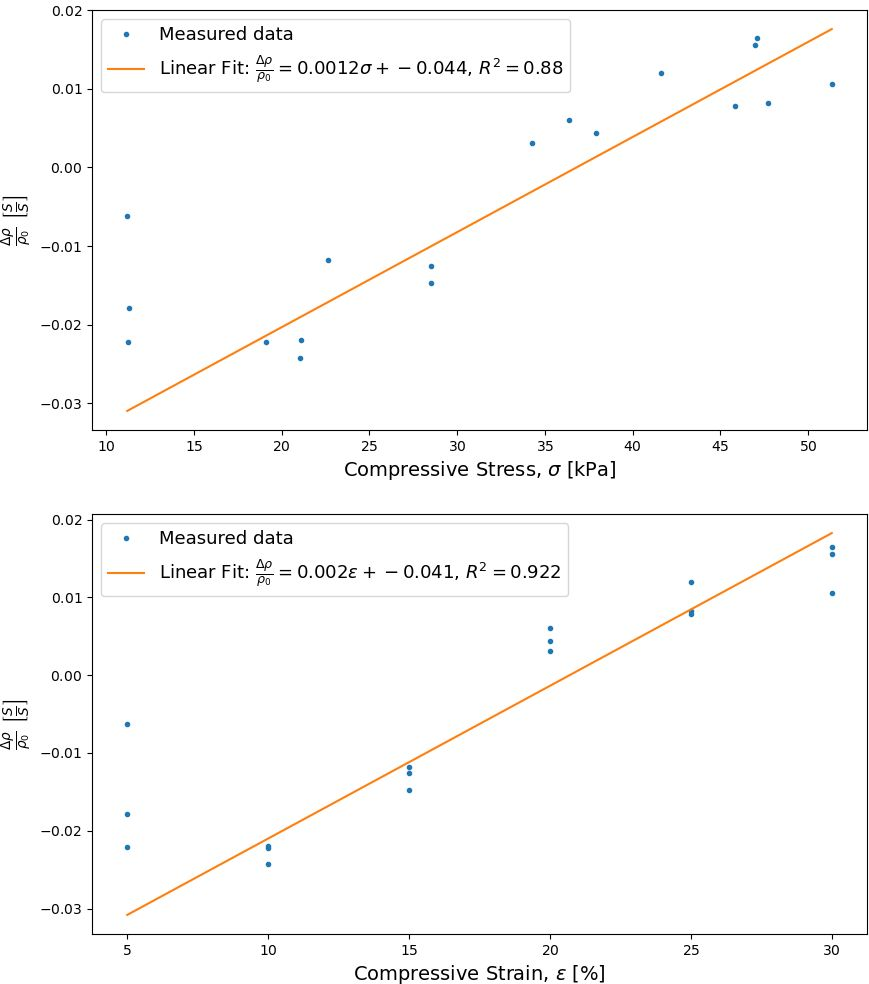
\includegraphics[width=0.7\linewidth]{Figures/CBSR_9p_cond_stress_strain_sin_titulo.jpg}
	\caption{Conductance change vs. stress (top) and strain (bottom) data and fitted curves for 9 wt\% CBSR. The 5\% strain values ignored as the $\mathrm{std}$ were larger than the conductance change values.}
	% TODO?: Change Linear fit to 10^{-1} from 10^{-3}
	\label{fig:quasi_r_9p}
\end{figure}

\section{1D and 2D Strain Settling Times}\label{apdx:Strain Relaxations}
\begin{figure}[H]
	\centering
	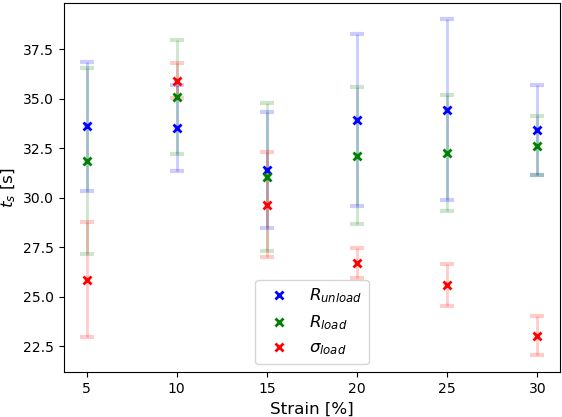
\includegraphics[width=0.8\linewidth]{Figures/CBSR_8p_1_10push_XXstrain_60s_ts_vals_vs_strain.jpg}
	\caption{Mean settling times for 5 - 30\% compressive strain applied to CBSR 8 wt\% with the error bars showing the standard deviation from 1D compressive test data.}
	\label{fig:strain_ts_8p_1D}
\end{figure}
\begin{figure}[H]
	\centering
	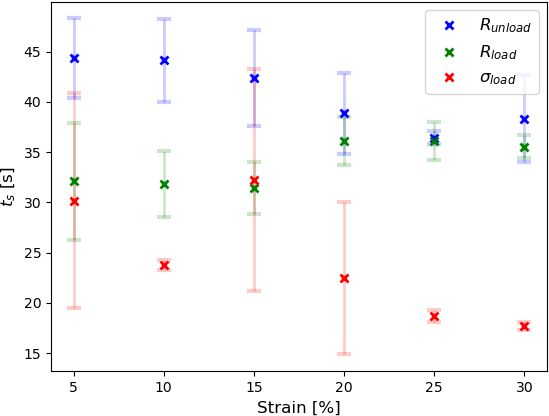
\includegraphics[width=0.8\linewidth]{Figures/CBSR_9p_1_3push_XXstrain_240s_ts_vals_vs_strain.jpg}
	\caption{Mean settling times for 5 - 30\% compressive strain applied to CBSR 9 wt\% with the error bars showing the standard deviation from 1D compressive test data.}
	\label{fig:strain_ts_9p_1D}
\end{figure}
\begin{figure}[H]
	\centering
	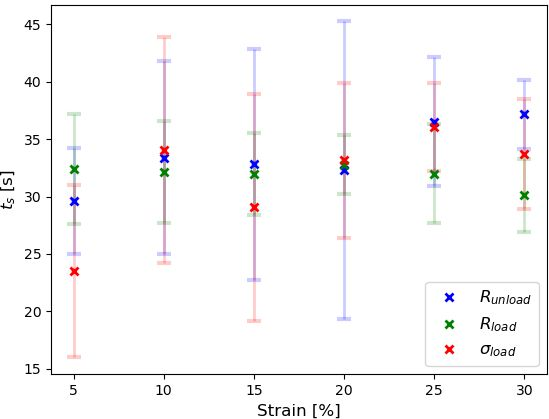
\includegraphics[width=0.8\linewidth]{Figures/CBSR_8p_1_9push_XXstrain_60s_X_ts_vals_vs_strain.jpg}
	\caption{Mean settling times for various strains applied to CBSR 8 wt\% with the error bars showing the standard deviation of each settling time from the 2D EIT experimental data.}
	\label{fig:strain_ts_8p}
\end{figure}
\begin{figure}[H]
	\centering
	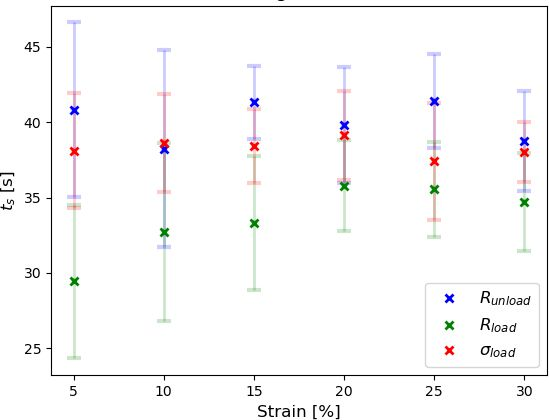
\includegraphics[width=0.8\linewidth]{Figures/CBSR_9p_2_9push_XXstrain_60s_1mA_X_ts_vals_vs_strain.jpg}
	\caption{Mean settling times for various strains applied to CBSR 9 wt\% with the error bars showing the standard deviation of each settling time from the 2D EIT experimental data.}
	\label{fig:strain_ts_9p}
\end{figure}


\section{Performance Metrics Example}\label{apdx:Performance Metrics}
\begin{figure}[H]
	\centering
	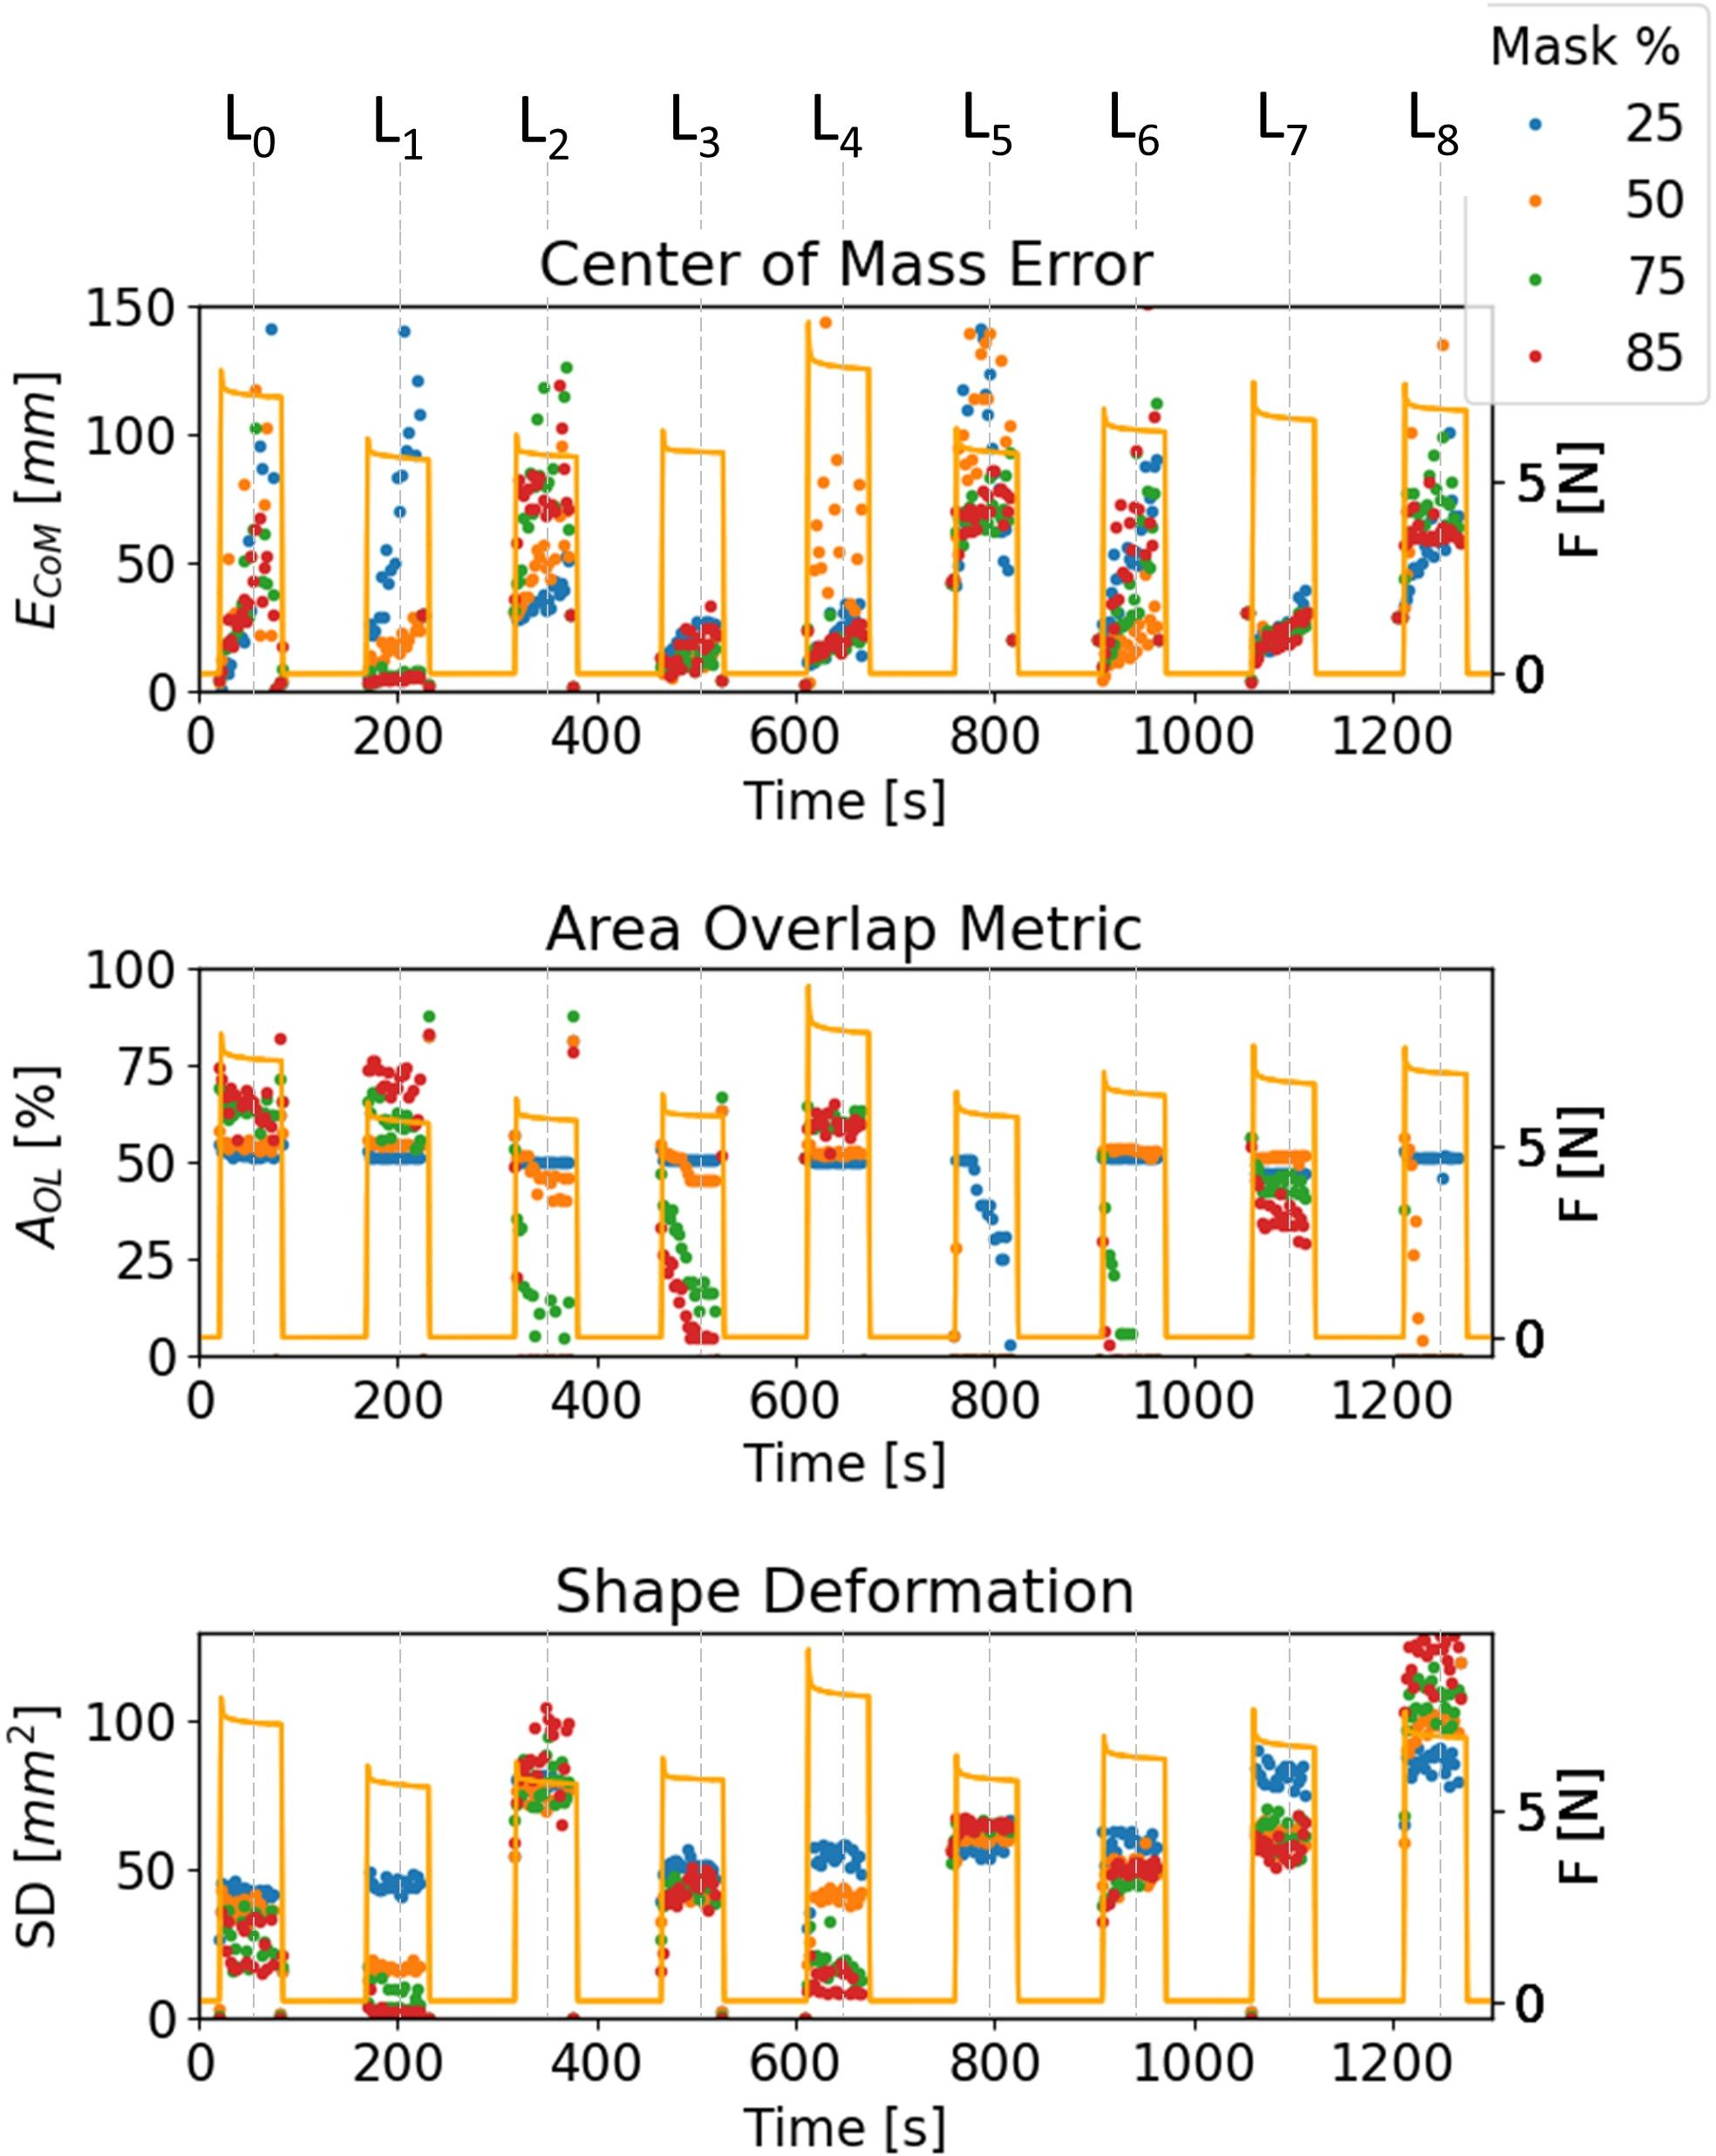
\includegraphics[width=0.8\linewidth]{Figures/CBSR_9p_9push_20strain_60s_4_metrics_thresh_masks_v2_numbd.jpg}
	\caption{Spatial performance metrics comparing threshold percentages of 25, 50, 75, and 85\% for 9 wt\% CBSR sample being loaded with 20\% compressive strain in nine areas, $L_{0-8}$, shown in Fig \ref{fig:force_app_map}.} % TODO?: Determine better way of displaying these metrics??
	\label{fig:recon_perform_9p}
\end{figure}

\section{Randomised test $S\!D$ metrics data}

\begin{table}[H]
	\caption{CBSR 8 and 9 wt\% mean and standard deviation for $S\!D$ spatial performance metrics of ten random locations, $L_{rand}$ and random strains $\varepsilon$}. % TODO: complete these tests with best blob algorithm??
	\label{tab:spatial_sd_metrics_stats_8p_rand_loads}
	\centering
	\hspace{0.4cm}
	\begin{tabular}{p{2.5cm}p{0.8cm}p{1.8cm}p{1.8cm}}
		\hline       
		$L_{rand}$(r, $\theta$) [mm, $\degree$] & $\varepsilon$ [\%] & 8wt\% $S\!D$ [mm] & 9wt\% $S\!D$ [mm] \\ \hline
		(5.4, 10) & 17.9 & 10.1 $\pm$ 0.8 & 9.8 $\pm$ 0.6\\
		(29.8, 337) & 24.0 & 62.2 $\pm$ 1.3 & 52.8 $\pm$ 1.3\\
		(4.2, 317) & 17.0 & 18.7 $\pm$ 5.9 & 21.7 $\pm$ 2.2\\
		(34.0, 70) & 10.9 & 20.2 $\pm$ 4.7 & 13.7 $\pm$ 0.8\\
		(35.8, 137) & 8.1 & 124.7 $\pm$ 2.8 & 81.5 $\pm$ 13.8\\
		(9.6, 55) & 13.8 & 24.8 $\pm$ 1.9 & 19.2 $\pm$ 1.8\\
		(2.8, 260) & 7.0 & 15.6 $\pm$ 4.5 & 12.7 $\pm$ 1.0\\
		(11.2, 114) & 10.0 & 4.5 $\pm$ 0.9 & 4.6 $\pm$ 0.6\\
		(24.6, 241) & 28.5 & 2.6 $\pm$ 0.1 & 2.6 $\pm$ 0.1\\
		(16.6, 253) & 23.6 & 0.3 $\pm$ 0.1 & 1.1 $\pm$ 0.1\\
		\hline
	\end{tabular}
\end{table}
	\chapter{Portable EIT-based Pressure Sensor Build and Operation}
\label{appendix-E}

This appendix is partially based on my HardwareX paper "A Portable Electrical Impedance Tomography Based Pressure Mapping Sensor and Validation System"\footnote{currently under review as of 26 September 2024} and gives a high-level description of the build process for both the ERT sensor module, the sensing domain, and the Cartesian force applicator (CFA). The build section are followed by an operation instructions and safety section.

\section{Build Methodology}
The build was split into two main parts the ERT sensor module electronics and the CFA construction. An example of how a piezoresistive nanoparticle elastomer composite is made is also re-iterated from previous chapters.


\subsection{ERT Sensor}
% grab gerber files send to PCB manufacturer. Place all SMD components. Place all THT components. Don't place jumpers until circuit has been tested. Copy and paste circuit test procedure. Place in housing for mounting on Prusa
The manufacturing process of the PCB involves first sending the PCB Gerber files to a PCB manufacturer. This work used JLC PCB with their default parameters for a 4 layer PCB.

Next populate the PCBs with the SMD parts given in the BOM and place in a reflow oven. First complete the rear side then the top side to ensure components stick. Once all SMD parts have been firmly soldered, solder all of the THT components. Finally attach the jumpers for the desired power mode, explained in Section \ref{sec:Operating modes}.
\begin{figure}[H]
	\centering
	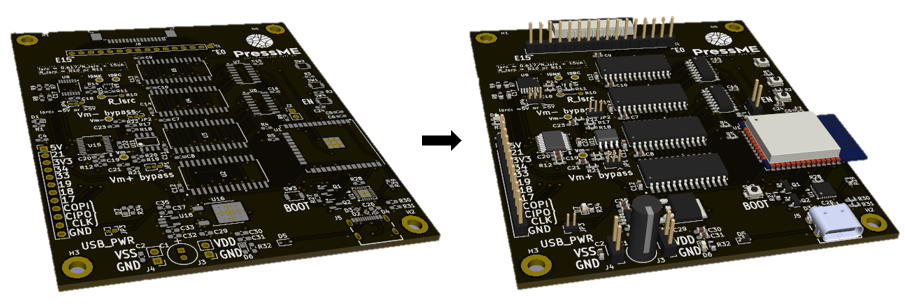
\includegraphics[width=0.8\linewidth]{Figures/HV_ERT_sensor_PCB_unpop2pop.png}
	\caption{ERT PCB [PCB1] before and after electrical component population.}
	\label{fig:pcb_to_pcba}
\end{figure}
To ensure simple protection against electrical shorts and low-level ingress protection (equivalent to IP20) 3D print an enclosure in PLA using the STL files given in the BOM, \textit{ert\_housing\_top.stl} [PR1]\footnote{Text within square brackets in this section refers to part reference designators (e.g. U1 for the ESP32 module) in the BOMs given in the supplementary material} and \textit{ert\_housing\_base.stl} [PR2]. There are 4 threaded inserts [HW2] to mount the PCB securely in the 3D printed enclosure using four M3 14 mm bolts [HW1].

Attach the 16 way ribbon connector [W1] to the ERT electrodes. In this example there is a ribbon to IDC connector interface board [J8], which then connects to a custom built electrode pin to domain interface [DUT1, DUT2, PR3, PR4]. This electrode interface will vary based on the required sensing domain.
\begin{figure}[H]
	\centering
	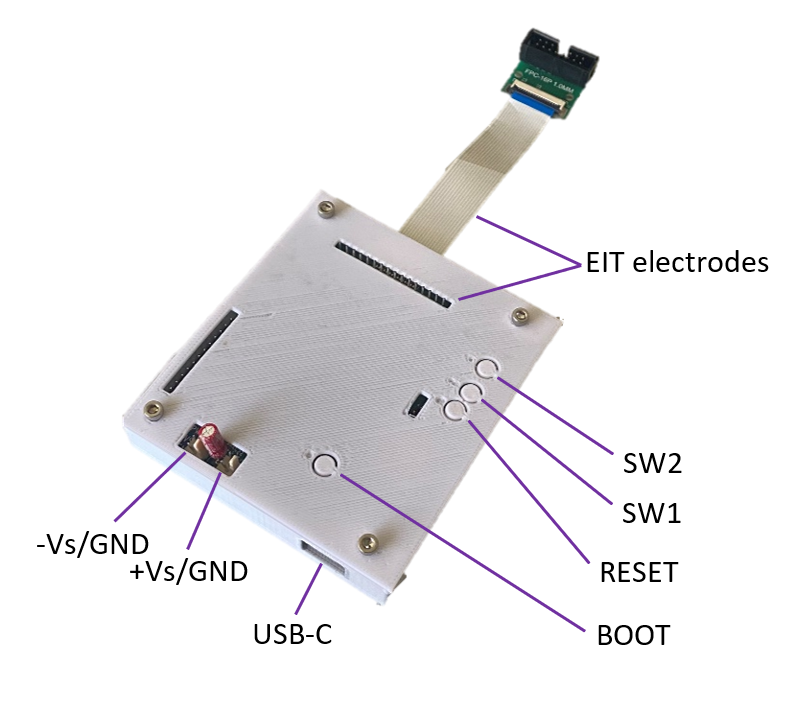
\includegraphics[width=0.6\linewidth]{Figures/ERT_PCB_assembled_in_housing_labelled.png}
	\caption{ERT sensor PCBA mounted in enclosure and attached electrode harness showing buttons and the main electrical connections.}
	\label{fig:ert_sensor_in_housing}
\end{figure}
The sensor device shown in Figure \ref{fig:ert_sensor_in_housing} shows all of the connections and buttons necessary for the programming and operation of the sensor, as well as two optional buttons SW1 and SW2 for any other desired functions.

\subsection{Sensing Domain}
\label{sec:Sensing Domain}
As a reference the method for fabricating a specific sensing domain is given in this section. The sensing domain used was a carbon black (CB) nanoparticle silicone rubber composite.

With the material requirements of a low Shore hardness of 5A - 25A, similar to that of human skin and muscle tissue \cite{Silvera-Tawil2015, Chatzistergos2022}, low viscoelasticity, high yield strength, low resistivity, high strain gauge factor, and non-toxic. Other sensor domain materials may be used for the sensor, such as soft conductive particle composites, conductive polymers, and hydrogels \cite{Giffney2017,Duan2014,Chen2023}.

Researchers fabricating their own sensing domain for use with this system should follow three key requirements, 
\begin{enumerate}
	\item The size of the sensing domain must fit within a 220 x 180 x 160 mm volume (X$\times$Y$\times$Z) on the CFA test bed. 
	\item The bulk modulus of the domain material must be chosen such that the required loads applied to the domain must not exceed 100 N.
	\item The inter-electrode resistance, $R_{int}$, must be low enough to not saturate the current source, $I_{src}$, given a power supply voltage, $V_s$, as shown in Equation \ref{eqn:r_int},
\end{enumerate}
\begin{equation}
	R_{int} < \alpha \frac{V_s}{I_{src}}
	\label{eqn:r_int}
\end{equation}
Where $R_{int}$ is the resistance values between every configuration of the current drive electrodes during an EIT capture cycle and $\alpha$ is the factor of safety for any electrode movement or incidental increase of $R_{int}$ during experimentation.

The domain under test (DUT) used in this work was a composite comprised of XC 72R carbon black (CB) nanoparticles (Cabot, Alpharetta, USA) [DUT5] of 50 nm average diameter, dispersed in a two part Dragon Skin 10 NV silicone rubber (SR) matrix (SmoothOn, Macungie, USA) [DUT6]. The weight percentage (wt\%) of CB to liquid silicone rubber which resulted in near optimal piezoresistive characteristics was found to be between 8 - 10\%. To ensure homogeneous CB particle dispersion and mitigate air bubble formation an ARV-310 vacuum planetary mixer (Thinky, Tokyo, Japan) was used to mix the CB particles through the liquid silicone matrix. Upon completion of mixing, the uncured composite was poured into the circular sheet domain mould. The curing of the composite was controlled by heating the newly-mixed material in the mould at 80$\degree$C for 90 min. The domain samples used in this work and previous work \cite{Ellingham2022, Ellingham2024} had a diameter of 100 mm as shown in Figure \ref{fig:CBSR_samples_examples}. 

\begin{figure}[H]
	\centering
	% 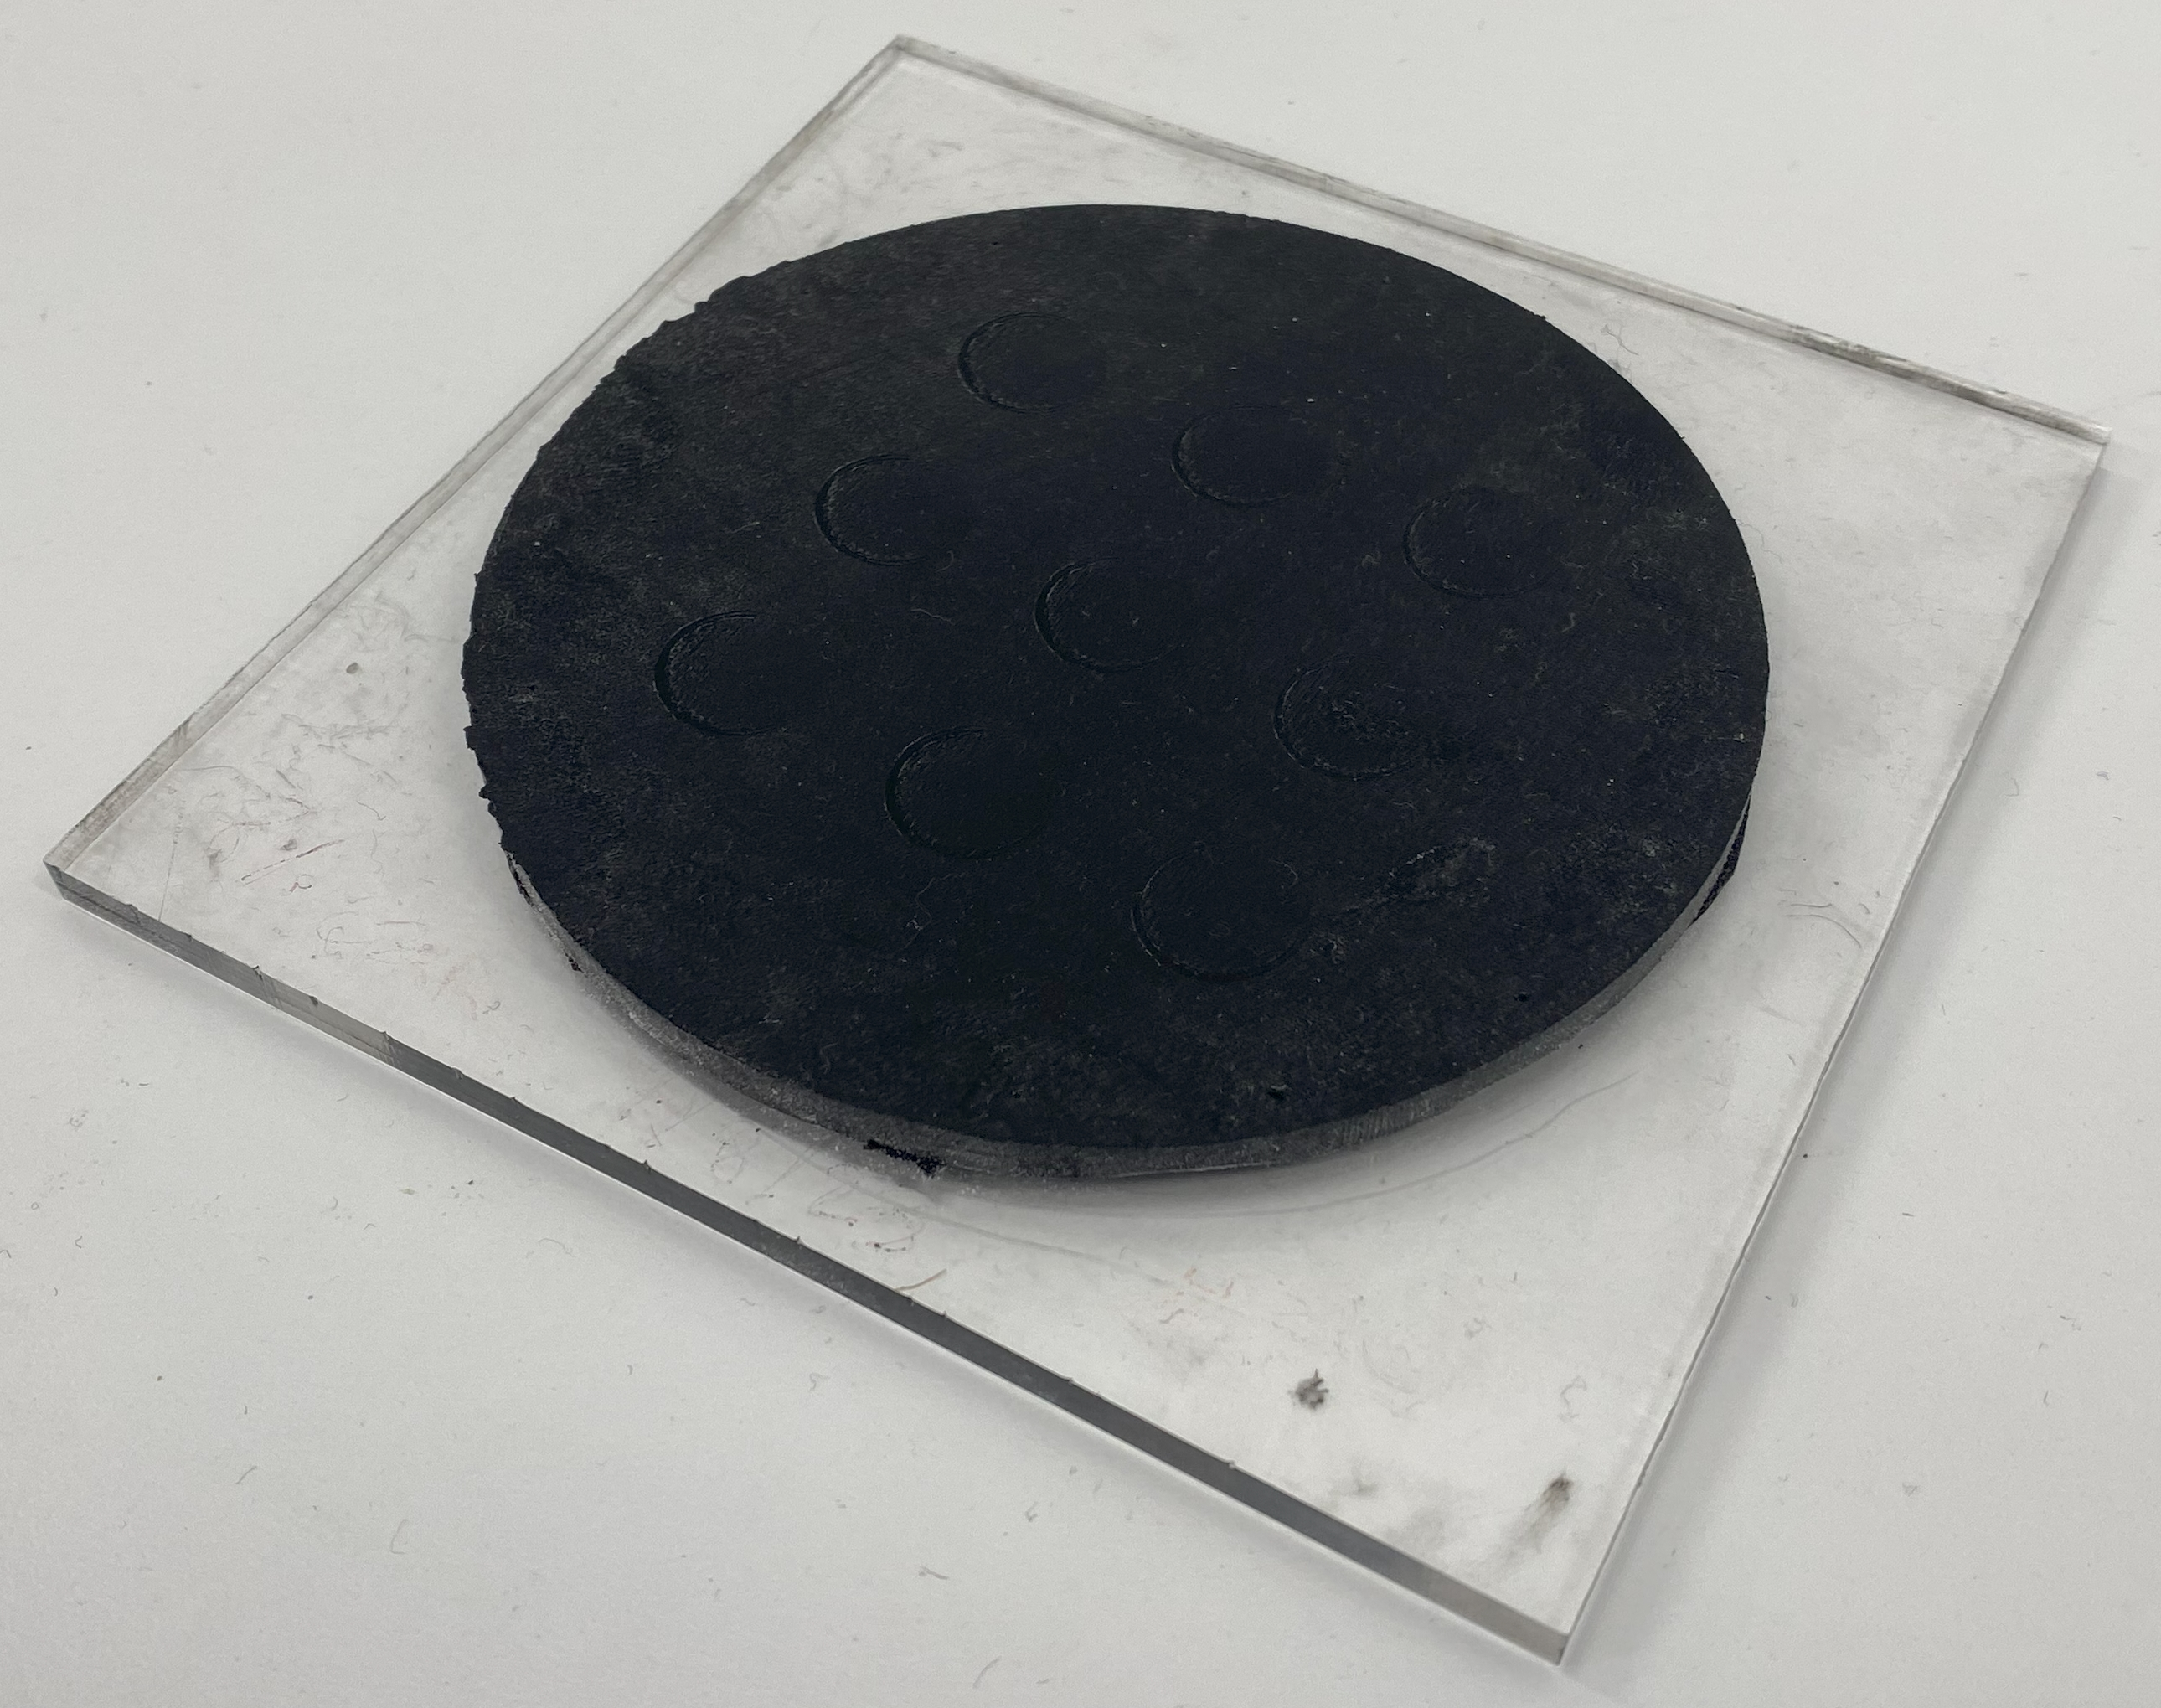
\includegraphics[width=0.295\linewidth]{Figures/CBSR_DUT_sample.jpg}
	% 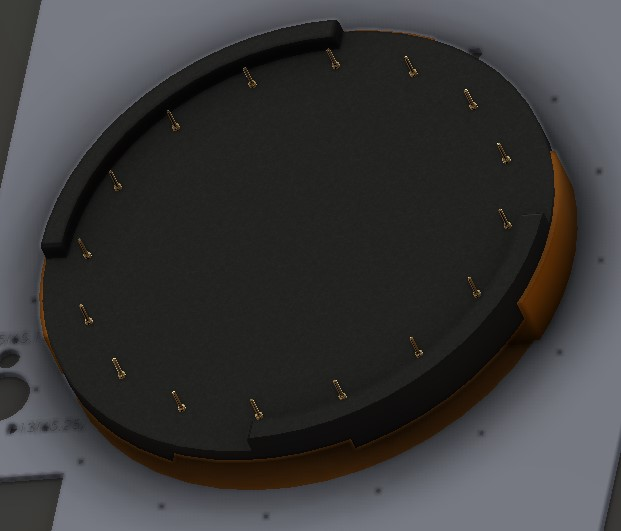
\includegraphics[width=0.275\linewidth]{Figures/ERT_sensing_domain_holder2.jpg}
	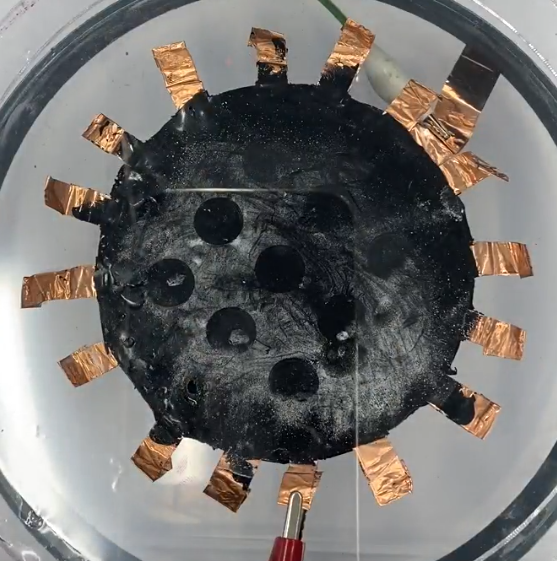
\includegraphics[width=0.3\linewidth]{Figures/DEA-EIT-sample_0.5mm_100mm.png}
	\hspace{2cm}
	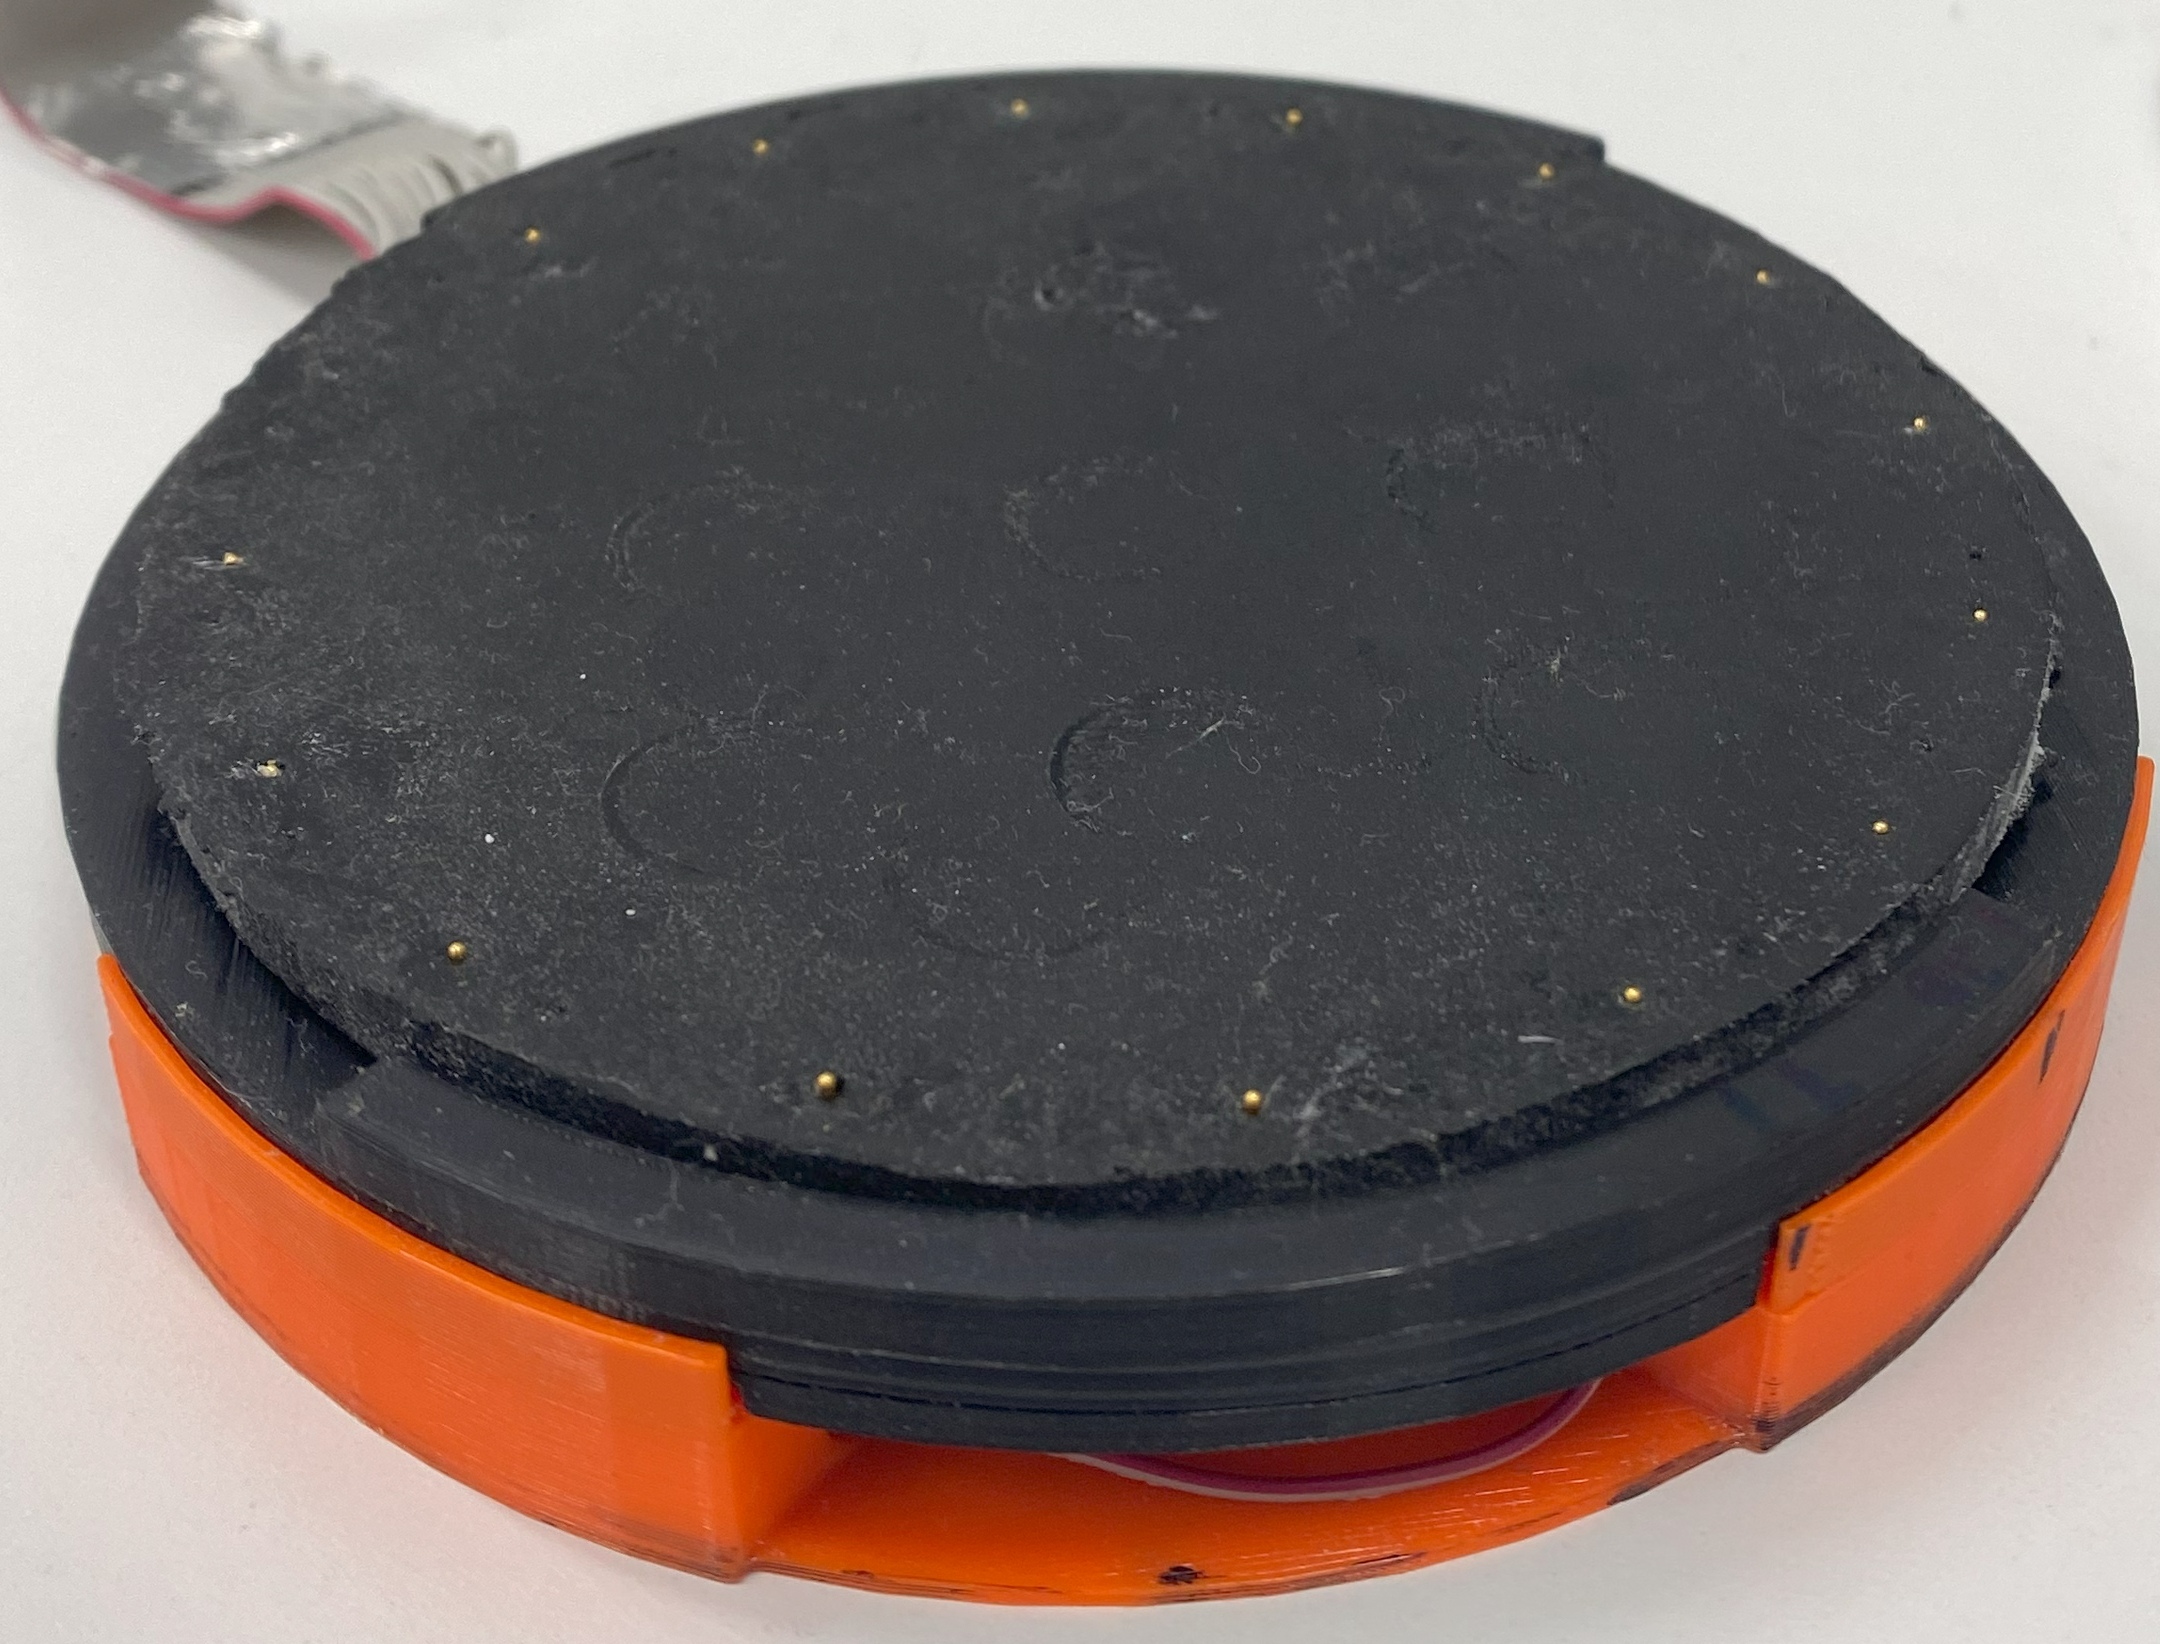
\includegraphics[width=0.4\linewidth]{Figures/CBSR_DUT_w_electrodes_sample.jpg}
	\caption{Left: An example of a CBSR sample with copper tape electrodes integrated with a dielectric elastomer actuator setup \cite{Ellingham2024a}. Right: Example of a CBSR sensing domain with gold pin electrodes penetrating material surface around the sensing region boundary.}
	\label{fig:CBSR_samples_examples}
\end{figure}


\subsection{Cartesian force applicator}
% Dismantle prusa printhead and trick thermistor. Mount loadcell, loadcell bridge, sensor tray, etc. Prepare sensing region surface...
To test the spatial and force resolution of the ERT pressure mapping device, the CFA was designed using a Prusa MK3s 3D printer to provide a stable platform. First a functional Prusa MK3s 3D printer was acquired with its printing capabilities tested on several standard demo PLA prints to ensure the print head can move with the expected resolution in the X, Y, and Z directions. Standard benchmark tests and tuning for the printing platform can be found  \href{https://blog.prusa3d.com/does-your-freshly-assembled-original-prusa-i3-mk3-print-as-the-best-it-can_29445/}{here} and \href{https://help.prusa3d.com/category/print-quality-troubleshooting_225}{here} \cite{Stritesky2019, Prusa2024}.

\begin{figure}[H]
	\centering
	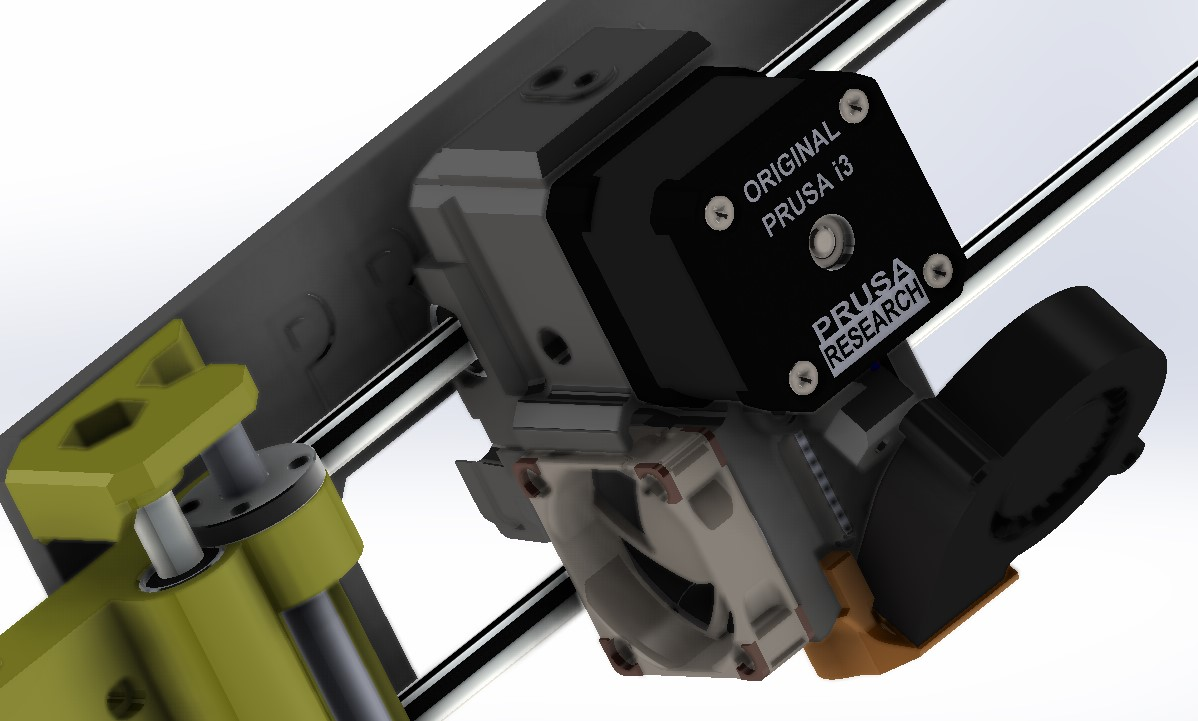
\includegraphics[width=0.4\linewidth]{Figures/og_MK3s_print_head.jpg}
	\hspace{1cm}
	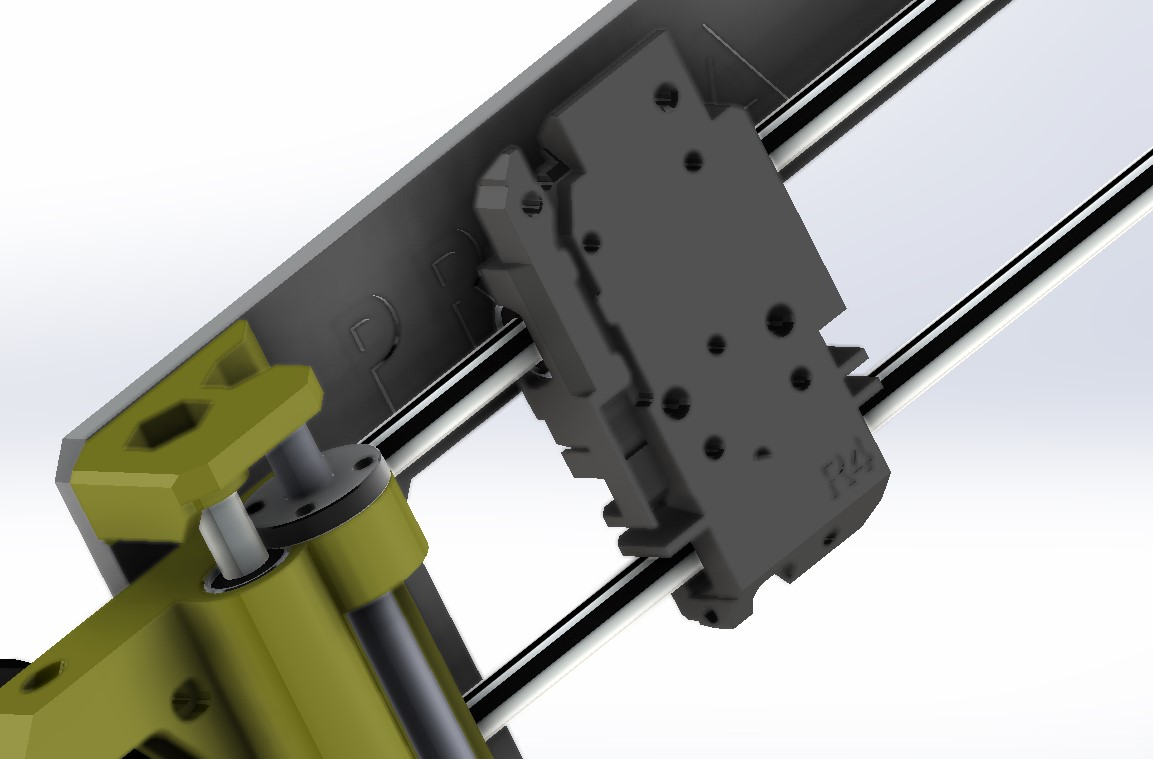
\includegraphics[width=0.4\linewidth]{Figures/dismantled_MK3s_print_head.jpg}
	% 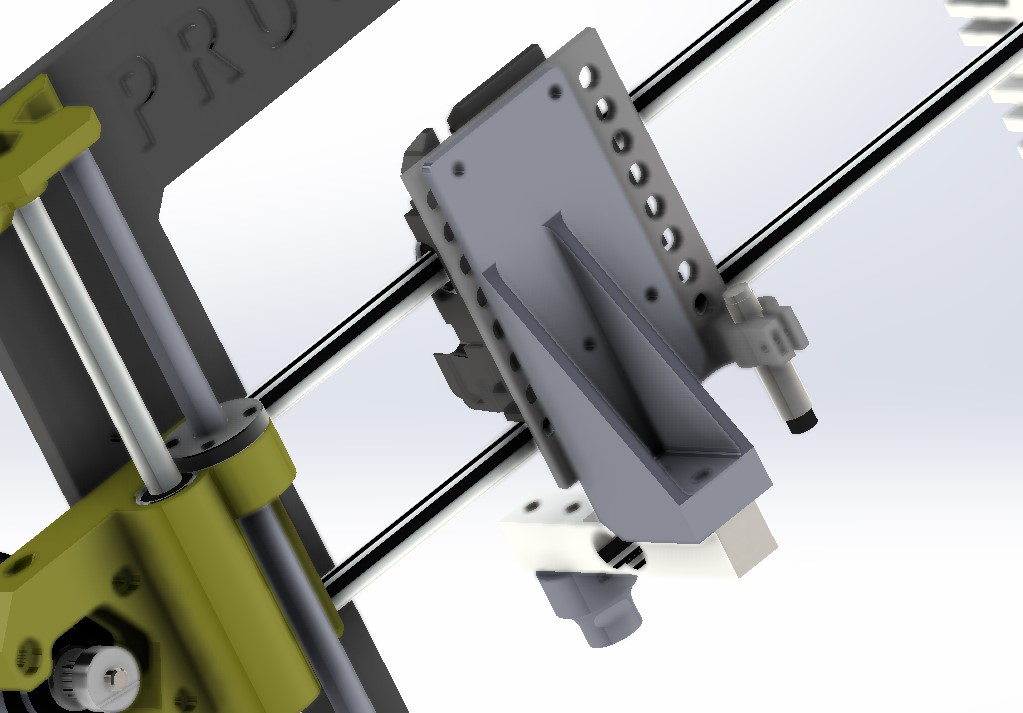
\includegraphics[width=0.32\linewidth]{Figures/modded_MK3s_print_head.jpg}
	\caption{MK3s print head. Left: Original print head assembly. Right: Dismantled print head assembly \cite{Kayne2019}.}
	\label{fig:mk3s_head_old_raw}
\end{figure}

Next the print head of the MK3s was dismantled, as shown in Figure \ref{fig:mk3s_head_old_raw}, leaving a flat surface to attach first the PINDA adaptor [PR8] and the loadcell bracket [PR9], as shown in Figure \ref{fig:mk3s_head_new}. Use M3 bolts to attach the loadcell bracket and PINDA adaptor to the dismantled print head surface. See read the printer \href{https://help.prusa3d.com/guide/5-e-axis-assembly_169235#170079}{assembly manual} for more detail on the part assembly\cite{Prusa2023}. Bolt the TAL220 10 kg loadcell [E3] onto the loadcell bracket using M5 bolts [HW4]. Bolt the force applicator head [PR5-7, HW5] onto the other end of the loadcell using M4 bolts [HW3]. A range of force applicator heads shapes and sizes have been created to test the resolution of the sensor. 
\begin{figure}[H]
	\centering
	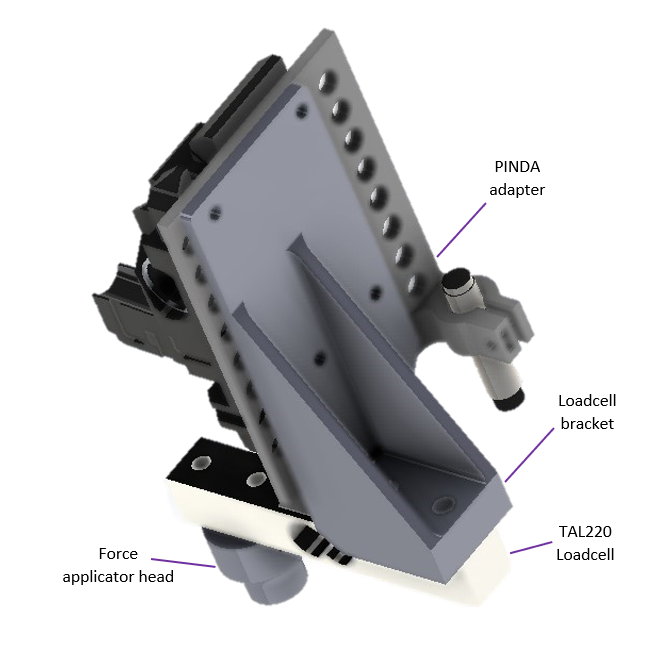
\includegraphics[width=0.5\linewidth]{Figures/modded_MK3s_print_head_clean_labelled.png}
	\caption{Force applicator head assembly.}
	\label{fig:mk3s_head_new}
\end{figure}
With the thermistor from the original printhead no longer required, a trimpot [RV1] is attached to the thermistor port on the printer's \href{https://help.prusa3d.com/guide/8-electronics-assembly_174100#175539}{control circuit PCBA}\cite{Prusa2023a}. While the 3D printer is turned on, the trimpot is manually adjusted until room temperature is reached on the 3D printer display to avoid any future under/over temperature errors.

The print bed of the MK3s 3D printer is removed and replaced with a mount tray [LC1] for the sensing domain. The ERT tray bearing part [PR10] mounted and bolted [HW6] onto the frame of the MK3s as shown in Figure \ref{fig:mk3s_new_trays}. The ERT sensor tray [LC2] and the sensing domain mount tray are fixed together onto the print bed with two M3 bolts [HW6] clamping the trays to the edge of the print bed.

\begin{figure}[H]
	\centering
	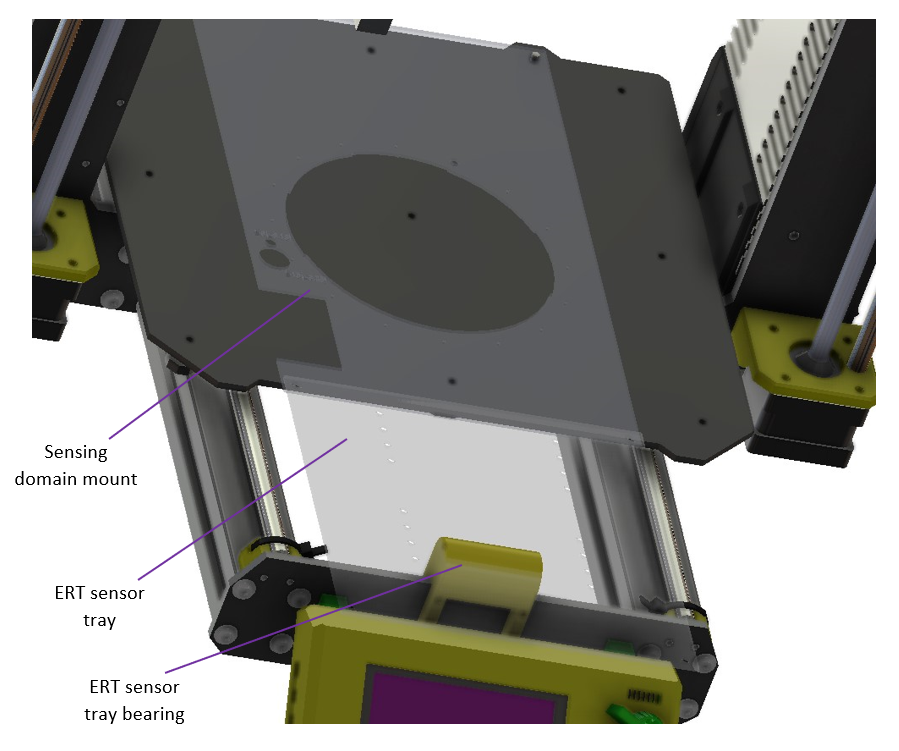
\includegraphics[width=0.6\linewidth]{Figures/cfa_trays_assm_labelled.png}
	\caption{MK3s with original print bed tray removed and the ERT sensor trays added.}
	\label{fig:mk3s_new_trays}
\end{figure}

The firmware version used in this work was MK3s 3.9.0. Later versions may be compatible. Other 3D printer platforms with a similar gcode command set and a similar core firmware such as the \href{https://marlinfw.org/}{Marlin firmware} may also be used as a CFA. However, minor configuration changes in this work's software and hardware may be required.

\section{Operation instructions}
%Provide detailed instructions for the safe and proper operation of the hardware. 
%> Step-by-step operational instructions for operating the hardware. 
%> Use visual instructions as necessary. 
%> Highlight potential safety hazards.
To validate and characterise the ERT pressure mapping sensor the CFA is used to apply a sequence of loads to the material. The below sequence of required operations to complete this experiment includes: 
\begin{enumerate}
	\item ERT sensor power modes
	\item ERT sensor programming
	\item ERT sensing domain preparation
	\item Load application point and strain configuration
	\item Touch based mesh bed levelling
	\item Load experiment execution
	\item Data capture
	\item Data processing
\end{enumerate}
This sequence of events is repeated for different sensing domains and different loading conditions.

\subsection{ERT sensor power modes}
\label{sec:Operating modes}
Before running any experiments, the ERT sensor power mode must be configured. The jumper configuration for the bipolar supply (blue) and +5 V USB single-ended supply (red) mode is shown in Figure \ref{fig:ert_pcb_pinout_mode}.

The bipolar supply first mode is recommended for driving the ERT signal through a wider range of sensing domains at a higher voltage. A bipolar supply of $\pm$20 V is connected to $\pm V_s$ for the best performance of the circuit.

The second power mode uses a +5 V USB 3.X power supply to run the ERT circuit. The second mode is limited to lower resistance sensing domains that can be tested as it can only drive constant currents using +5 V. When using the +5 V supply mode the $-V_s$ and GND pins on the power input must be shorted for the multiplexers to operate. 
\begin{figure}[H]
	\centering
	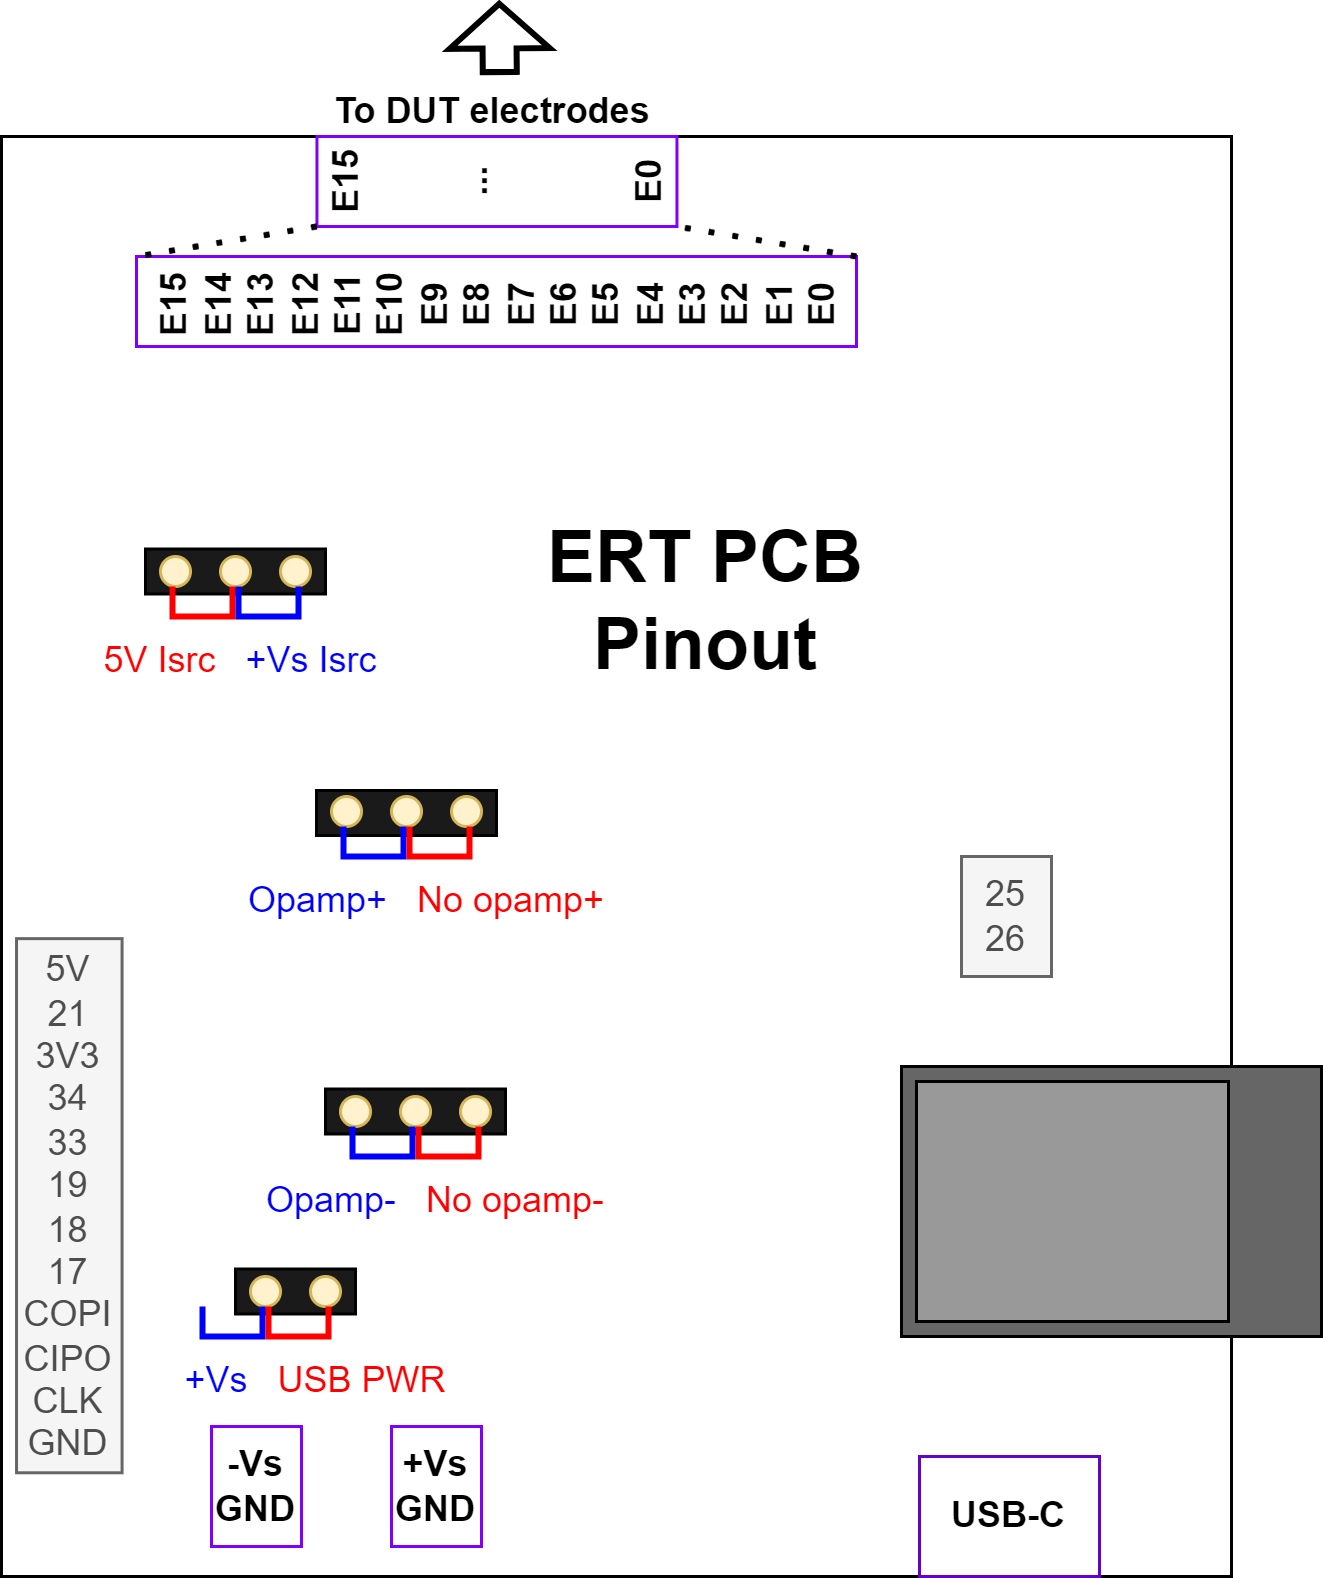
\includegraphics[width=0.3\linewidth]{Figures/ert_pcb_pinout.png}
	\caption{ERT PCB pin-out and power mode options. Blue jumpers are for the bipolar supply mode (i.e. $\pm V_s$ attached). Red jumpers are for the +5 V USB supply mode. }
	\label{fig:ert_pcb_pinout_mode}
\end{figure}
For each power mode there will be a distortion of the signal dependent on the power supply voltages and input signal as exemplified in Figure \ref{fig:mux_r_on}.


\subsection{ERT sensor programming}
The ERT sensor contains an ESP-WROOM32 module [U1] which requires the \verb|main_ert.c| program to be built and flashed. This can be achieved using the default project template from the \href{https://docs.espressif.com/projects/esp-idf/en/stable/esp32/get-started/index.html}{ESP-IDF environment}\cite{Espressif2024}. The default ERT circuit firmware \verb|main_ert| completes the well proven adjacent electrode drive pattern \cite{Avis1992,Xu2008,Dang2021,Zamora-Arellano2020}. Upon successful programming of the ERT circuit it will output a constant serial stream of the adjacent electrode pattern ERT data separating each frame of 256 measurements with an `\verb|A|'. The ERT sensor circuit has the capability to send the real-time serial ERT data via a USB serial, Bluetooth, or WiFi connection to a EIT reconstruction capable computer.


\subsection{ERT sensing domain preparation}
For sensing domain fabrication instructions refer to Section \ref{sec:Sensing Domain}. The ERT sensing domain needs to have sufficiently low adjacent inter-electrode resistance to function, so that the current source will not saturate due the power supply voltage. The ET electrodes can be attached to the domain in many ways as shown in Figure \ref{fig:CBSR_samples_examples}, ensure these connections provide a reliable electrical contact to the sensing domain. Connect sensing domain electrodes to the ERT circuit FPC connector[W1] via an adaptor[J8]. The ERT sensing domain must be flat and centred on the sensing domain holder [PR3, PR4] as shown in Figure \ref{fig:CBSR_samples_examples} (middle). 


\subsection{Load application point and strain configuration}
Load application points and strains applied to the sensing domain can be configured by altering variables in \verb|ertpcb_cfa_reader.py| code. A loading sequence consists of a series of load applications, in the form of a strain pulse train, applied to a set of X and Y coordinates on the sensing domain. The main parameters to change for running a loading sequence are given in Table \ref{tab:ert_cfa_params}.
\begin{table}[H]
	\caption{CFA experimental parameter variables.}
	\label{tab:ert_cfa_params}
	\begin{tabular}{|p{0.3\linewidth}|p{0.1\linewidth}|p{0.5\linewidth}|}
		\hline
		\textbf{Variable:}  & \textbf{Unit:} & \textbf{Description:} \\ \hline
		Strain speed (\texttt{v\_z\_push}) & mm/min & The rising/falling edge gradient for each pulse. \\ \hline
		Strain limit (\texttt{strain\_limit}) & \% & The maximum compressive strain allowed. \\ \hline
		Load locations (\texttt{push\_points}) & [mm, mm] & An array of XY locations of each load pulse. \\ \hline
		Reference offset (\texttt{ref\_loc\_mm}) & [mm, mm] & The XY offset of the zero point of the sensing domain relative to the CFA home reference. \\ \hline
	\end{tabular}
\end{table}
% \begin{itemize}
	%     \item Push time [s] - The time each strain pulse is held for.
	%     \item Strain displacement speed [mm/min] - The rising/falling edge gradient for each pulse.
	%     \item Load locations [mm, mm] - the xy locations of each load pulse.
	%     \item Strain values [\%] - The strain values of each load pulse. 
	%     \item Sample thickness [mm] - The sample domain thickness
	%     \item Current source [A] - The constant current source value.
	% \end{itemize}
These can all be found as variables in the software file \verb|ertpcb_cfa_reader.py| within the \verb|main| function. Before running this program the serial COM ports may need to be changed in the \verb|ertpcb_cfa_reader.py| program to match the comports of the CFA and ERT sensor hardware.

\subsection{Load experiment execution}
Once all hard-coded parameters have been set the command parameters are set and the load experiment begins. To begin the load experiment use the following terminal command:
\begin{verbatim}
	>> python ertpcb_cfa_reader.py <dir/filename> <Isrc_A> <Vmax> <sample_name> <date_fabricated>
\end{verbatim}
\vspace{-1cm}
\begin{verbatim}
	<load_time_s> <strain>
\end{verbatim}

Where \verb|<dir/filename>| is includes the file directory and file name, \verb|<Isrc_A>| is the constant current source value set in the ERT circuit in amps, \verb|<Vmax>| is the maximum allowed voltage to be read by the ADC in volts (e.g. 20 V), \verb|<sample_name>| is a descriptive sensing domain name, \verb|<date_fabricated>| is the sample fabrication date (`NA' or leave blank if irrelevant), \verb|<load_time_s>| is the strain pulse on and off time in seconds, and \verb|<strain>| is the desired strain applied to the domain as a percentage. If a random test sequence is desired with randomised strain and locations this can be achieved by simply setting the \verb|<strain>| value to -1.


\subsection{Touch-based mesh bed levelling}
% if sample isn't perfectly flat mesh bed leveling can compensate.
An undulating sensing domain surface can often be present during testing due to an intentionally curved sensor or manufacturing defects. To compensate for an uneven surface a touch-based mesh bed levelling process has been created to improve the quality of the stress/strain data gathered. The process involves the force applicator head travelling towards the sample until a change in force has been detected above 0.1 N. This mitigates the risk of any misalignment with the force applicator surface plane and the sensing domain surface plane and ensures more accurate strain data capture for low strain magnitudes. This touch-based mesh bed levelling is completed before the load sequence experiment begins. The sensing domain and holding trays should not be physically contacted in any form after beginning the \verb|ertpcb_cfa_reader.py| program.


\subsection{Data capture}
Once the \verb|ertpcb_cfa_reader.py| program has completed capturing data, a time-series plot of the 16 inter-electrode resistances, $R_{int}$, will appear. A stable $R_{int}$ is for stable EIT reconstructions of the sensing domain.  

Any significant change in the inter-electrode resistance may cause a poor EIT reconstruction result. A significant change in the inter-electrode resistance could be a result of, applying force too close to the electrodes themselves, an inherently unstable electrode connection, or an external force applied near the electrode. If the $R_{int}$ values are not stable it will be evident in the plot and there will be a warning message in the console. 
\begin{figure}[H]
	\centering
	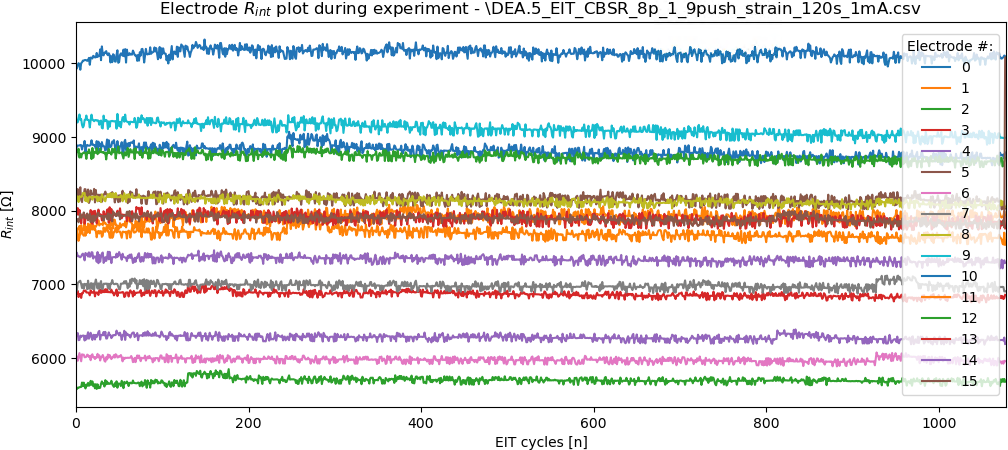
\includegraphics[width=0.8\linewidth]{Figures/Rint_plot.png}
	\caption{An example plot of the $R_{int}$ values generated on completion of an experiment for a stable experiment. Where the Electrode \# `i' represents the resistance between electrode `i' and `i+1'.}
	\label{fig:ert_pcb_pinout_mode}
\end{figure}
Once the inter-electrode resistance plot is closed the program will continue to save all of the data in three separate files for the given \verb|filename|,
\begin{enumerate}
	\item \textit{filename}.csv - Time series data for ERT voltages, compression forces, and force applicator XYZ locations. The UTC start date and time of the experiment is given in the top row.  
	\item \textit{filename}.pkl - Logs the same data as the .csv file \textbf{and} all of the important experiment parameters into a serialised python `pickle' file.
	\item \textit{filename}.gcode - The gcode file of the commands sent to the 3D printer platform for the experiment run.
\end{enumerate}


\subsection{Data processing}
% Default EIT reconstruction algorithm (don't need to provide this)
Once all of the data has been collected in the above steps, the data can be processed. Data processing includes the following,
\begin{enumerate}
	\item Pre-processing of the raw voltage, force, and position data. Filtering and data cleaning could be included in this step.
	\item Image reconstruction using a chosen EIT algorithm with the pre-processing or raw data. EIT reconstruction could include algorithms such as regularised Newton's methods \cite{Lionheart2003}, neural network based methods \cite{Biasi2022, Husain2021}, and back projection methods \cite{Avis1992}.
	\item Any post-processing of the EIT image reconstruction data and integration with the force applicator stress and/or strain data. Post-processing could include resistance to force inverse modelling, pressure mapping performance metric quantification, an application specific software interface.
\end{enumerate}
In this work EIDORS \cite{Sherry2006} has been used to complete the EIT reconstructions of the domain and any post processing is then completed with a python program as shown in Section \ref{sec:Validation and characterisation}.


\section{Construction and Operational Safety}
Various safety concerns must be stated for the construction and operation precautions of this system. This is not a comprehensive safety guide, but will give an overview of some potential safety concerns. Other precautions may be necessary depending on the development location and sensing domain materials used. The construction and operation of the system can each be separated into three parts, the ERT sensor circuit, the CFA, and the sensing domain.


\subsection{Construction}
During the assembly of the ERT sensor circuit the regular health and safety procedures for assembling and soldering a PCB must be followed.

During testing of the CFA as a 3D printer there will be moving parts which could get caught on long hair or collide with a person too close. Steps must be taken to avoid any undesired collisions or any people touching the CFA during operation.

When fabricating the sensing domain often this involves micro/nano sized conductive particles dangerous for inhalation and sometimes dangerous to touch. The material safety datasheet must be consulted for any material used in the sensing domain. Any safety procedures with mixing machines and curing devices must be followed.

\subsection{Operation}
The PCBA can operate on up to $\pm$ 20 VDC which is within the safe level the SELV as defined by IEC \cite{IEC2005}. However, should the contacts of the power supply to the ERT circuit be electrically shorted, a burn or fire hazard may arise. The current on the sensing domain electrodes is limited to prevent a dangerous short circuit current.

During the operation of the CFA there will be moving parts which could collide tangle long hair or collide with the person operating. Steps must be taken to avoid any undesired collisions or any people touching the CFA during operation.

The sensing domain may not be bio-compatible so the material safety datasheet(s) for each domain must be followed for each real world sensor application.

	\chapter{Dielectric Elastomer Generator Validation}
\label{appendix-F}

\section{$\Delta V$ Calculcation}
An estimate of the ideal voltage, $\Delta V$, generated from a circular compression load of radius, $r_L$, on a circular DE domain of radius, $r_{DE}$, with two conductive compliant electrodes covering the area $A_{DE}$ of the DE.

Several assumptions are made to simplify the calculation to be solved analytically:
\begin{enumerate}
	\item The capacitance of the unloaded system is made up of the base DE capacitance.
	\item The capacitance of the loaded system is a summation of the base DE capacitance and loaded area capacitance.
	\item The parallel plate capacitor assumptions are made for both DE and loaded area capacitances.
	\item The relative permittivity of the DE remains constant with changing strain.
\end{enumerate}

The dependent parameters voltage, $\Delta V$, and energy, $\Delta U$, generated by the DEG are a result of the change in the DE capacitance, the charge, $Q$, on the DE electrodes, and the physical parameters of the DE. The independent physical parameters of the DE system include:
\begin{itemize}
	\item $A_{DE}$ - area of the dielectric elastomer capacitance
	\item $d_i$ - relaxed DE thickness
	\item $\epsilon_r$ - relative permittivity of free space
	\item $V_i$ - initial priming voltage input
	\item $Q$ - DE charge
\end{itemize}
The parameters independent parameters for driving energy generation include:
\begin{itemize}
	\item $\varepsilon$ - compressive strain of the load applied
	\item $A_L$ - area of the applied load
\end{itemize}

Using Equations \ref{eqn:elastic-energy} - \ref{eqn:elec-energy2} as a basis for the DEG method, we form a formula for the voltage generated $\Delta V$, based on the priming voltage, $V_i$ and the stage two voltage, $V_{ii}$ as,
\begin{equation}
	\Delta V = V_{ii} - V_i = \frac{Q}{C_{i}} - \frac{Q}{C_{ii}}.
	\label{eqn:F1}
\end{equation}
Which then can be rearranged to obtain a formula for $\Delta V$ as a function of $C$ and $V_i$,
\begin{equation}
	\Delta V = V_i \left(\frac{C_{ii}}{C_i} - 1\right)
	\label{eqn:F2}
\end{equation}

For a load with a strain, $\varepsilon$, we get a compressed DE thickness $d_{ii}$ such that,

\begin{equation}
	d_{ii} = d_i(\varepsilon + 1).
	\label{eqn:F3}
\end{equation}

Substituting the parallel capacitance formulae for $C_i$ and $C_{ii}$ we get,

\begin{equation}
	C_i = \frac{\epsilon (A_{DE})}{d_i}
	\label{eqn:F4}
\end{equation}
and
\begin{equation}
	C_{ii} = \frac{\epsilon (A_{DE} - A_L)}{d_i} + \frac{\epsilon A_L}{d_{ii}}
	\label{eqn:F5}
\end{equation}

where $\epsilon = \epsilon_0\epsilon_r$. By substituting Equations \ref{eqn:F3} - \ref{eqn:F5} into Equation \ref{eqn:F2} we can obtain an analytical solution for the system. 

For a more accurate analytical solution utilising surface integrals and Maxwell's equations could be used on a case by case basis for different loads. However this approach has not been used as each deriving each analytical solution is cumbersome and not extendable for a range of load shapes that may be experienced in real world scenarios.



		
	\addtocontents{toc}{\vspace{2em}}  % Add a gap in the Contents, for aesthetics
	\backmatter
	%% ----------------------------------------------------------------
	\label{Bibliography}
	\lhead{\emph{Bibliography}}  % Change the left side page header to "Bibliography"
	\bibliographystyle{unsrtnat}  % Use the "unsrtnat" BibTeX style for formatting the Bibliography
	\bibliography{Bibliography}  % The references (bibliography) information are stored in the file named "Bibliography.bib"
\end{document}  % The End
%% ----------------------------------------------------------------